% arxiv_template.tex
% Custom LaTeX template for Quarto → arXiv-style PDF output.
% This replaces Quarto's default Pandoc template.
% Pandoc variables are injected via  syntax.

\documentclass{article}

% ── Core packages ──────────────────────────────────────────────────────────────
\usepackage{arxiv}            % arXiv style — upload arxiv.sty to project root
\usepackage[utf8]{inputenc}
\usepackage[T1]{fontenc}
% Map Unicode Greek letters to LaTeX math equivalents (for pdflatex)
\DeclareUnicodeCharacter{03B1}{\ensuremath{\alpha}}
\DeclareUnicodeCharacter{03B2}{\ensuremath{\beta}}
\DeclareUnicodeCharacter{03B3}{\ensuremath{\gamma}}
\DeclareUnicodeCharacter{03B4}{\ensuremath{\delta}}
\DeclareUnicodeCharacter{03B5}{\ensuremath{\varepsilon}}
\DeclareUnicodeCharacter{03B7}{\ensuremath{\eta}}
\DeclareUnicodeCharacter{03BA}{\ensuremath{\kappa}}
\DeclareUnicodeCharacter{03BC}{\ensuremath{\mu}}
\DeclareUnicodeCharacter{03C1}{\ensuremath{\rho}}
\DeclareUnicodeCharacter{03C3}{\ensuremath{\sigma}}
\DeclareUnicodeCharacter{03C4}{\ensuremath{\tau}}
\DeclareUnicodeCharacter{03C6}{\ensuremath{\phi}}
\DeclareUnicodeCharacter{2212}{\ensuremath{-}}   % U+2212 MINUS SIGN
\DeclareUnicodeCharacter{2264}{\ensuremath{\leq}}
\DeclareUnicodeCharacter{2265}{\ensuremath{\geq}}
\usepackage{amsmath, amssymb, amsfonts}
\usepackage{bm}
\usepackage{graphicx}
% Constrain all figures to fit within the text column.
% Fixes "Overfull \hbox" warnings from wide PNG/raster figures.
% Quarto 3.x's \pandocbounded{} is a no-op; this rule does the actual work.
\setkeys{Gin}{width=\linewidth,totalheight=\textheight,keepaspectratio}
\usepackage{booktabs}
\usepackage{longtable}
\usepackage{array}
% calc + xfp are required for Pandoc's proportional column-width formula:
%   p{(\linewidth - N\tabcolsep) * \real{0.25}}
% Without them, any multi-column auto-width table triggers a
% "Missing number, treated as zero" fatal LaTeX error.
\usepackage{calc}
\usepackage{xfp}
\usepackage{multirow}
\usepackage{float}
\usepackage{caption}
\usepackage{subcaption}
\usepackage{algorithm}
\usepackage{algorithmic}
\usepackage{nicefrac}
\usepackage{microtype}
\usepackage{setspace}
\usepackage{xcolor}
\usepackage{enumitem}
\usepackage[most]{tcolorbox}
\usepackage{fontawesome5}
\definecolor{quarto-callout-note-color}{HTML}{4582EC}
\definecolor{quarto-callout-note-color-frame}{HTML}{4582EC}
% geometry already loaded by arxiv.sty — do not reload

% ── Citations ──────────────────────────────────────────────────────────────────
\usepackage{natbib}
\bibliographystyle{unsrtnat}

% ── Cross-referencing ──────────────────────────────────────────────────────────
\usepackage{hyperref}
\usepackage{cleveref}
\hypersetup{
  colorlinks=true,
  linkcolor=blue,
  urlcolor=blue,
  citecolor=blue,
  pdftitle={Dissociating Perseverative Responding from Learning-Rate
Effects in Trauma: A Computational Modeling Approach},
  pdfauthor={Jasmine Burrows, Adam Manoogian},
}

% ── Float spacing ─────────────────────────────────────────────────────────────
\setlength{\intextsep}{8pt plus 2pt minus 2pt}
\setlength{\floatsep}{8pt plus 2pt minus 2pt}
\setlength{\textfloatsep}{10pt plus 2pt minus 2pt}

% ── Pandoc parskip fix ────────────────────────────────────────────────────────
% arxiv.sty sets \parskip=5.5pt (sized for hand-written LaTeX with few blank
% lines). Pandoc/Quarto emits blank lines around every equation, figure, and
% section, and each one becomes a \par that adds 5.5pt of spurious vertical
% space — producing visible "gaps" above/below equations and floats.
% Override to a small stretch-only value so structural LaTeX spacing
% (\intextsep, \floatsep, amsmath's \abovedisplayskip) controls layout.
\usepackage{etoolbox}
\setlength{\parskip}{0pt plus 1pt}
\AtBeginEnvironment{figure}{\setlength{\parskip}{0pt}}
\AtBeginEnvironment{figure*}{\setlength{\parskip}{0pt}}

% ── Author block ──────────────────────────────────────────────────────────────
\usepackage{authblk}
\renewcommand\Authfont{\bfseries}
\setlength{\affilsep}{0em}

% ── ORCID icon ────────────────────────────────────────────────────────────────
% Place orcid.pdf in manuscript/ for ORCID icons next to author names
\newbox{\orcidbox}
\IfFileExists{orcid.pdf}{%
  \sbox{\orcidbox}{\includegraphics[scale=0.06]{orcid.pdf}}%
}{%
  \sbox{\orcidbox}{}% no icon if file missing
}

% ── Title / authors (injected by Quarto) ─────────────────────────────────────
\title{Dissociating Perseverative Responding from Learning-Rate Effects
in Trauma: A Computational Modeling Approach}

\author[uts]{%
  %
  Jasmine Burrows%
  %
}
\author[mc3s,mbi,turner]{%
  \href{https://orcid.org/0009-0002-8002-3191}{\usebox{\orcidbox}\hspace{1mm}}%
  Adam Manoogian%
  \thanks{\texttt{adam.manoogian@monash.edu}}%
}

\affil[uts]{University of Technology Sydney}
\affil[mc3s]{Monash Centre for Consciousness and Contemplative Studies,
Monash University}
\affil[mbi]{Monash Biomedical Imaging, Monash University}
\affil[turner]{Turner Institute for Brain and Mental Health, Monash
University}

% ── Pandoc internals ──────────────────────────────────────────────────────────
\providecommand{\tightlist}{%
  \setlength{\itemsep}{0pt}\setlength{\parskip}{0pt}}
\providecommand{\pandocbounded}[1]{#1}  % Pandoc 3.x image wrapper


% ── Document ──────────────────────────────────────────────────────────────────
\begin{document}
\maketitle

\begin{abstract}
Trauma exposure alters reinforcement learning (RL) and working memory
(WM) processes, but the computational mechanisms remain unclear. We
fitted seven computational models, spanning classical Q-learning (M1),
WM-RL hybrids with optional perseveration kernels (M2, M3, M5, M6a,
M6b), and a joint choice-plus-response-time model using a Linear
Ballistic Accumulator (M4), to data from 162 participants completing a
reinforcement learning working memory task. The preferred model by both
AIC and BIC was M6b, which decomposes perseverative responding into
choice-level and stimulus-level components via a stick-breaking share
parameter (\(\kappa_{\text{share}}\)). Parameter-recovery simulations on
synthetic data show that the two perseveration parameters
(\(\kappa_{\text{total}}\), \(\kappa_{\text{share}}\)) are identifiable
(\(r \geq 0.93\)), but the base RLWM parameters (learning rates, WM
decay, WM reliability, capacity, attentional noise) fall short of the
\(r \geq 0.80\) criterion. Trauma-parameter associations were marginal:
the strongest effects were a positive association between the
perseveration kernel (\(\kappa_{\text{total}}\), M6b; \(\kappa\), M3)
and lifetime trauma exposure (LEC-5 Total Events), which survived
false-discovery-rate correction only in M3. We report all associations
alongside uncorrected, FDR-BH, and Bonferroni-corrected p-values and
situate the findings as hypothesis-generating, pending confirmation in
an independent sample.
\end{abstract}

\keywords{reinforcement learning \and working
memory \and trauma \and perseveration \and computational
psychiatry \and PTSD}

\section{Introduction}\label{sec-intro}

Trauma exposure produces lasting changes in learning and decision-making
that extend well beyond the initial stressor
\citep{lissek2005classical, homan2019neural}. Computational psychiatry
has begun to characterize these changes in terms of reinforcement
learning (RL) parameters: altered learning rates, impaired value
representations, and disrupted prediction-error signals
\citep{browning2015anxious, gillan2016characterizing, millner2018pavlovian}.
Yet a fundamental ambiguity remains: apparent learning-rate deficits
following trauma may reflect not genuine insensitivity to outcomes, but
rather motor perseveration --- a tendency to repeat prior actions
independent of their value.

Working memory (WM) contributes substantially to behavior on RL tasks,
particularly at low set sizes where stimuli fit within WM capacity
\citep{collins2012how, collins2014working}. The WM-RL hybrid model of
\citet{senta2025} formalizes this interaction and introduces a
perseveration parameter (\(\kappa\)) that captures action repetition
tendencies separable from outcome-based learning. By applying this
framework to a trauma-exposed sample, we can ask whether post-reversal
failures following trauma reflect elevated \(\kappa\) (motor habit),
reduced \(\alpha\) (outcome insensitivity), or both.

This paper describes the fitting of seven hierarchically nested
computational models (M1 Q-learning through M6b dual-perseveration) to
behavioral data from 162 participants stratified by trauma history and
post-traumatic stress symptom severity. We compare models by AIC/BIC,
identify the winning model, and examine how its parameters relate to
trauma group membership and continuous symptom measures from the IES-R
\citep{weiss2007impact} and LEC-5 \citep{weathers2013life}.

\section{Methods}\label{sec-methods}

\subsection{Participants}\label{sec-participants}

Participants were included in all downstream analyses only if they met
the v4.0 canonical inclusion criteria implemented in
\texttt{config.get\_analysis\_cohort()}, which enforces the intersection
of three gates: (1) \textbf{task completeness} --- at least 400 trials
and at least eight main-task blocks; (2) a \textbf{performance check}
--- overall accuracy above 0.40 AND mean accuracy over the last 5
main-task blocks above 0.50 (the late-block criterion confirms the
participant learned rather than performing at or near chance throughout
the session, since chance = 1/3 \(\approx\) 0.333); (3) \textbf{scale
completeness} --- non-missing values on every required survey column
(LEC-5 total events, IES-R total, IES-R intrusion, IES-R avoidance,
IES-R hyperarousal). The resulting analysis cohort comprised
\textbf{162} participants. Trauma exposure and symptom severity were
assessed via the Life Events Checklist for DSM-5 (LEC-5;
\citet{weathers2013life}) and the Impact of Event Scale--Revised (IES-R;
\citet{weiss2007impact}). Participants were classified into two groups
based on LEC-5 endorsement and IES-R total score: \textbf{Trauma - No
Ongoing Impact} (n = 63) and \textbf{Trauma - Ongoing Impact} (n = 114).

Scale distributions and pairwise correlations are summarized in
Figure~\ref{fig-scale-distributions}.

\begin{figure}[H]

\centering{

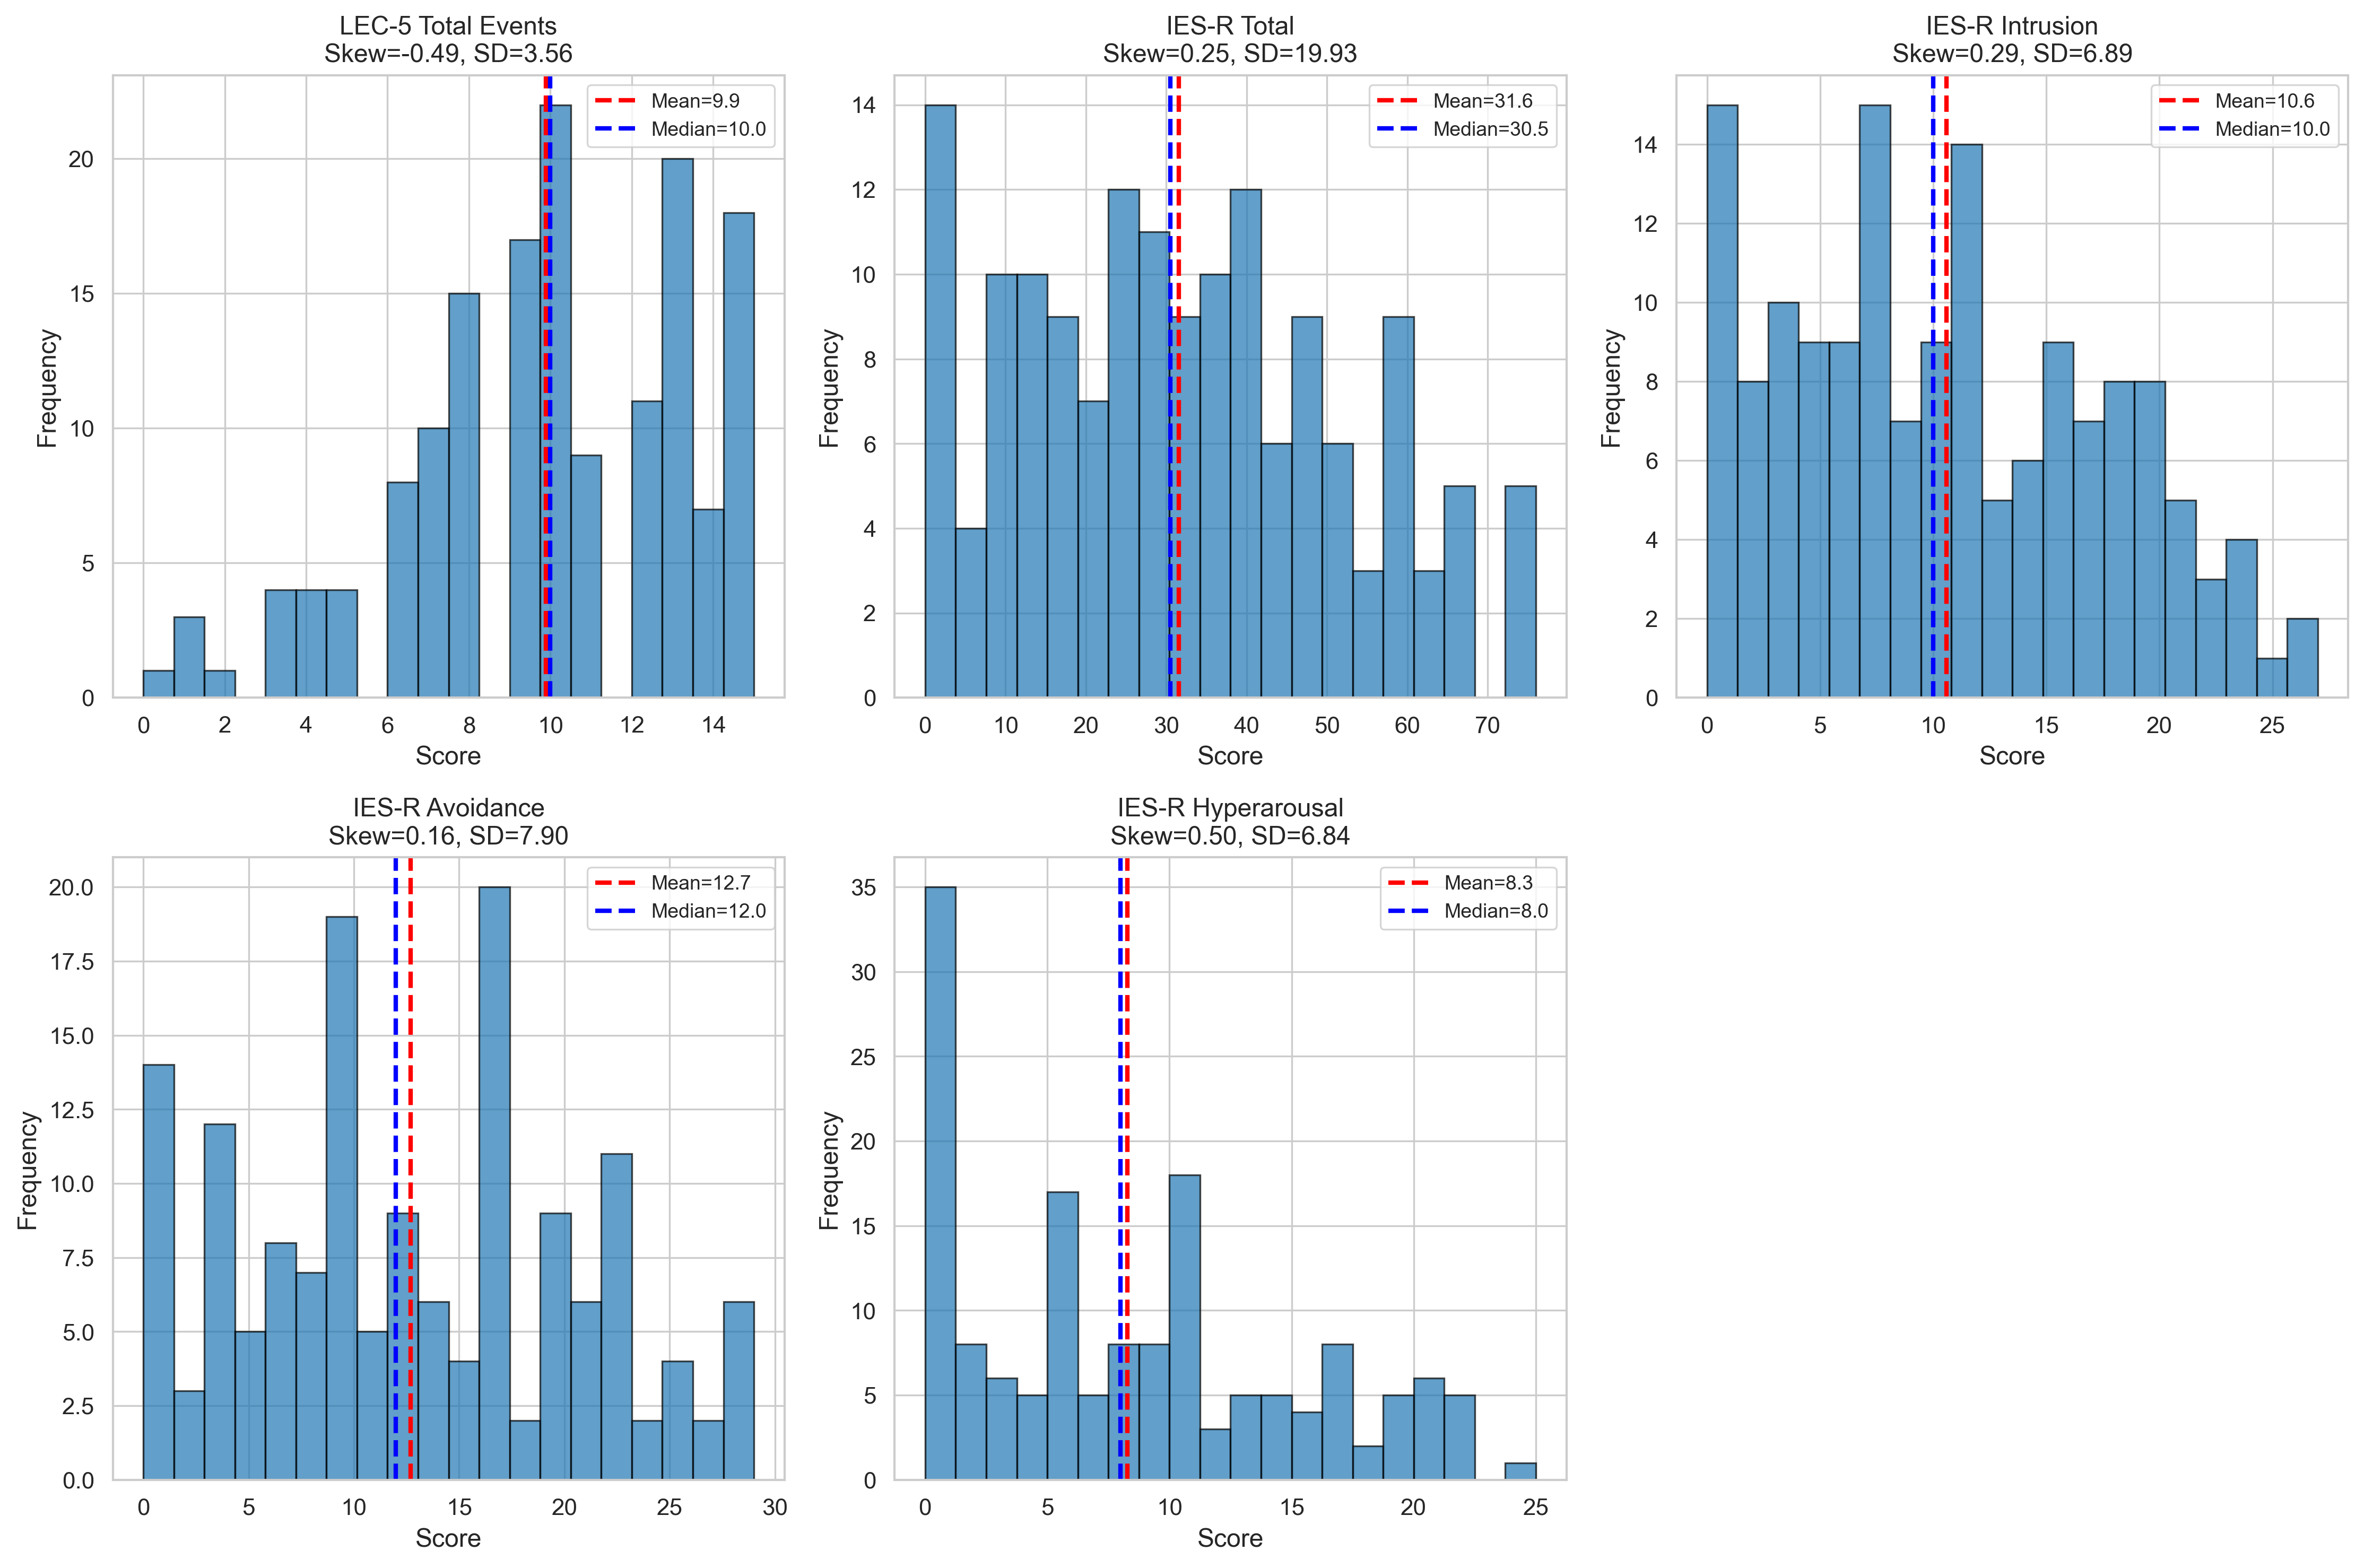
\includegraphics[width=1\linewidth,height=\textheight,keepaspectratio]{figures/scale_distributions.png}

}

\caption{\label{fig-scale-distributions}Distributions and pairwise
correlations of the trauma predictors. \textbf{Left}: histograms of
LEC-5 total events and IES-R total and subscale scores. \textbf{Right}:
Pearson correlation matrix. LEC total correlates only weakly with IES
total (\(r\) = 0.13), justifying inclusion of both predictors. IES
subscales correlate strongly with IES total (\(r\) = 0.91--0.93),
requiring the Gram--Schmidt residualization described in Model Fitting.
Figure source: \texttt{manuscript/figures/scale\_distributions.png}.}

\end{figure}%

\subsection{Task}\label{sec-task}

Participants completed the RLWM task from \citet{senta2025} implemented
in jsPsych. On each trial, a stimulus was presented and participants
selected one of three response options (J, K, L) using the keyboard.
Feedback (correct/incorrect) was provided after each response. Stimuli
were organized into blocks with set sizes of 2, 3, 5, or 6 stimuli (set
size 4 excluded), with rare reversals of correct response mappings
occurring after 12--18 consecutive correct responses. The task comprised
two practice blocks (static and dynamic) followed by up to 21 main-task
blocks (see Section~\ref{sec-exclusions} for inclusion thresholds).

\subsection{Computational Models}\label{sec-models}

We fitted seven models of increasing complexity to each participant's
trial-by-trial choices (see Section~\ref{sec-model-table} for complete
parameter listings). All WM-RL models share a core architecture in which
behaviour arises from a mixture of reinforcement learning (RL) and
working memory (WM) policies, with the WM contribution weighted by
capacity and set size.

\textbf{Core WM-RL architecture.} On each trial, WM decays globally
toward a uniform baseline, then overwrites the observed
stimulus--action--reward association:
\[\text{WM}(s,a) \leftarrow (1 - \phi)\,\text{WM}(s,a) + \phi / n_A
\qquad\text{(decay)},\qquad
\text{WM}(s,a) \leftarrow r
\qquad\text{(update)}\] RL values are updated via an asymmetric delta
rule: \[Q(s,a) \leftarrow Q(s,a) + \alpha\,\delta, \qquad
\delta = r - Q(s,a)\] Both systems produce softmax choice probabilities
(\(\beta = 50\), fixed), combined via an adaptive weight:
\[\omega = \rho \cdot \min\!\left(1,\; K / n_s\right),\qquad
p_{\text{hybrid}}(a \mid s) = \omega\,p_{\text{WM}} + (1-\omega)\,p_{\text{RL}}\]

\textbf{Epsilon noise and dual perseveration (M6b).} The winning model
adds uniform noise and two perseveration kernels (global and
stimulus-specific) via a stick-breaking parameterization:
\[\kappa = \kappa_{\text{total}} \cdot \kappa_{\text{share}}, \qquad
\kappa_s = \kappa_{\text{total}} \cdot (1 - \kappa_{\text{share}})\] The
final choice probability is:
\[p(a \mid s) = (1 - \kappa - \kappa_s)\left[\frac{\varepsilon}{n_A} + (1-\varepsilon)\,p_{\text{hybrid}}\right]
+ \kappa\,\mathbf{1}[a = a_{\text{last}}]
+ \kappa_s\,\mathbf{1}[a = a_{\text{last}}^{(s)}]\] where
\(a_{\text{last}}\) is the globally previous action and
\(a_{\text{last}}^{(s)}\) is the previous action for stimulus \(s\).

\begin{tcolorbox}[enhanced jigsaw, arc=.35mm, bottomrule=.15mm, bottomtitle=1mm, breakable, colback=white, colbacktitle=quarto-callout-note-color!10!white, colframe=quarto-callout-note-color-frame, coltitle=black, left=2mm, leftrule=.75mm, opacityback=0, opacitybacktitle=0.6, rightrule=.15mm, title=\textcolor{quarto-callout-note-color}{\faInfo}\hspace{0.5em}{Model Parameter Glossary}, titlerule=0mm, toprule=.15mm, toptitle=1mm]

\textbf{Learning rate.} \(\alpha\) governs the speed of Q-value updates
following prediction errors. A single symmetric learning rate is used
for both positive and negative prediction errors.

\textbf{WM decay} (\(\phi\)). Controls how rapidly WM representations
degrade between trials. Higher \(\phi\) means faster information loss
from working memory, forcing greater reliance on the slower RL system.

\textbf{WM reliability} (\(\rho\)). Scales the overall contribution of
WM to the action policy. Lower \(\rho\) means the participant relies
less on WM even when capacity permits it.

\textbf{WM capacity} (\(K\)). The number of stimulus-response mappings
that can be actively maintained in working memory. When \(K \geq n_s\),
WM can represent all stimuli in the block; when \(K < n_s\), WM coverage
is partial.

\textbf{Perseveration} (\(\kappa\)). A tendency to repeat previous
actions independent of their expected value. M3 uses a single global
\(\kappa\); M6a uses a stimulus-specific \(\kappa_s\); M6b decomposes
perseveration into a total budget \(\kappa_{\text{total}}\) allocated
between global and stimulus-specific components via a share parameter
\(\kappa_{\text{share}}\) (stick-breaking parameterization).

\textbf{RL forgetting} (\(\phi_{\text{RL}}\), M5 only). Decays Q-values
toward the uniform baseline (\(1/n_A\)) before each update, capturing
forgetting of non-attended stimulus values in the RL system.

\textbf{Noise} (\(\varepsilon\)). Probability of a uniformly random
response, capturing motor noise or inattention:
\(p_{\text{noisy}}(a) = \varepsilon / n_A + (1 - \varepsilon) \cdot p(a)\).

The inverse temperature \(\beta = 50\) is fixed for identifiability
\citep{senta2025}.

\end{tcolorbox}

The six choice-only models (M1--M3, M5, M6a, M6b) are compared by AIC
and BIC. M4 (RLWM-LBA) uses a joint choice-plus-RT likelihood and cannot
be compared by AIC with choice-only models; it is evaluated on a
separate track.

{

\begin{longtable}[]{@{}
  >{\raggedright\arraybackslash}p{(\linewidth - 16\tabcolsep) * \real{0.1111}}
  >{\raggedright\arraybackslash}p{(\linewidth - 16\tabcolsep) * \real{0.1111}}
  >{\raggedright\arraybackslash}p{(\linewidth - 16\tabcolsep) * \real{0.1111}}
  >{\raggedright\arraybackslash}p{(\linewidth - 16\tabcolsep) * \real{0.1111}}
  >{\raggedright\arraybackslash}p{(\linewidth - 16\tabcolsep) * \real{0.1111}}
  >{\raggedright\arraybackslash}p{(\linewidth - 16\tabcolsep) * \real{0.1111}}
  >{\raggedright\arraybackslash}p{(\linewidth - 16\tabcolsep) * \real{0.1111}}
  >{\raggedright\arraybackslash}p{(\linewidth - 16\tabcolsep) * \real{0.1111}}
  >{\raggedright\arraybackslash}p{(\linewidth - 16\tabcolsep) * \real{0.1111}}@{}}

\caption{\label{tbl-model-architecture}Free parameters across the seven
computational models. A checkmark indicates the parameter is estimated
in that model; empty cells indicate the parameter is not included. Rows
are grouped by functional role (learning rates, working memory,
perseveration, RL forgetting, noise, LBA dynamics). The inverse
temperature \(\beta = 50\) is fixed across all models for
identifiability. M1--M6b are choice-only and compared by AIC/BIC; M4
(joint choice-plus-RT) uses a Linear Ballistic Accumulator likelihood
and is evaluated on a separate track.}

\tabularnewline

\toprule\noalign{}
\begin{minipage}[b]{\linewidth}\raggedright
Group
\end{minipage} & \begin{minipage}[b]{\linewidth}\raggedright
Parameter
\end{minipage} & \begin{minipage}[b]{\linewidth}\raggedright
M1
\end{minipage} & \begin{minipage}[b]{\linewidth}\raggedright
M2
\end{minipage} & \begin{minipage}[b]{\linewidth}\raggedright
M3
\end{minipage} & \begin{minipage}[b]{\linewidth}\raggedright
M5
\end{minipage} & \begin{minipage}[b]{\linewidth}\raggedright
M6a
\end{minipage} & \begin{minipage}[b]{\linewidth}\raggedright
M6b
\end{minipage} & \begin{minipage}[b]{\linewidth}\raggedright
M4
\end{minipage} \\
\midrule\noalign{}
\endhead
\bottomrule\noalign{}
\endlastfoot
Learning rate & \(\alpha\) & \(\checkmark\) & \(\checkmark\) &
\(\checkmark\) & \(\checkmark\) & \(\checkmark\) & \(\checkmark\) &
\(\checkmark\) \\
Working memory & \(\phi\) & & \(\checkmark\) & \(\checkmark\) &
\(\checkmark\) & \(\checkmark\) & \(\checkmark\) & \(\checkmark\) \\
Working memory & \(\rho\) & & \(\checkmark\) & \(\checkmark\) &
\(\checkmark\) & \(\checkmark\) & \(\checkmark\) & \(\checkmark\) \\
Working memory & \(K\) & & \(\checkmark\) & \(\checkmark\) &
\(\checkmark\) & \(\checkmark\) & \(\checkmark\) & \(\checkmark\) \\
Perseveration & \(\kappa\) & & & \(\checkmark\) & \(\checkmark\) & & &
\(\checkmark\) \\
Perseveration & \(\kappa_{s}\) & & & & & \(\checkmark\) & & \\
Perseveration & \(\kappa_{\mathrm{total}}\) & & & & & & \(\checkmark\)
& \\
Perseveration & \(\kappa_{\mathrm{share}}\) & & & & & & \(\checkmark\)
& \\
RL forgetting & \(\phi_{\mathrm{RL}}\) & & & & \(\checkmark\) & & & \\
Noise & \(\varepsilon\) & \(\checkmark\) & \(\checkmark\) &
\(\checkmark\) & \(\checkmark\) & \(\checkmark\) & \(\checkmark\) & \\
LBA (M4 only) & \(v_{\mathrm{scale}}\) & & & & & & & \(\checkmark\) \\
LBA (M4 only) & \(A\) & & & & & & & \(\checkmark\) \\
LBA (M4 only) & \(\delta\) & & & & & & & \(\checkmark\) \\
LBA (M4 only) & \(t_{0}\) & & & & & & & \(\checkmark\) \\
& \(k\) (total) & 2 & 5 & 6 & 7 & 6 & 7 & 9 \\

\end{longtable}

}

\begin{figure}[H]

\centering{

\pandocbounded{\includegraphics[keepaspectratio]{paper_files/figure-pdf/fig-param-distributions-output-1.pdf}}

}

\caption{\label{fig-param-distributions}Distribution of key parameter
estimates across choice-only models. Violins show the full distribution
across 162 participants. Shared parameters are plotted for each model
that includes them.}

\end{figure}%

\subsection{Model Fitting}\label{sec-fitting}

Each model was fitted to each participant's main-task trials by maximum
likelihood estimation (MLE) using scipy's L-BFGS-B optimizer with 50
random restarts per participant. Likelihoods were computed via
JAX-accelerated functions with GPU support on the Monash M3 cluster.
Frequentist model comparison used the Akaike Information Criterion:
\(\text{AIC} = 2k - 2\ln\hat{L}\), where \(k\) is the number of free
parameters \citep{daw2011model}, and the Bayesian Information Criterion:
\(\text{BIC} = k\ln(n) - 2\ln\hat{L}\).

To obtain full posterior distributions and principled uncertainty
propagation, we additionally fitted all seven models using hierarchical
Bayesian inference in NumPyro \citep{phan2019composable} with the
No-U-Turn Sampler (NUTS; \citet{hoffman2014no}). Participant
log-likelihoods were attached to the model via \texttt{numpyro.factor}
and evaluated in parallel across posterior samples using
\texttt{jax.vmap}. Individual-level parameters were given non-centered
parameterizations following the hBayesDM convention
\citep{ahn2017revealing}: \(\theta_i = l + (u - l) \cdot \Phi(\mu +
\sigma \cdot z_i)\), where \(\Phi\) is the standard normal CDF,
\(\mu \sim
\mathcal{N}(\mu_0, 1)\) is the group-level location, \(\sigma \sim
\text{HalfNormal}(0.2)\) is the group-level scale, and \(z_i \sim
\mathcal{N}(0, 1)\) is the individual offset. Trauma associations were
estimated as Level-2 shifts on the unconstrained (probit) scale:
\(\mu_{\text{shifted}} = \mu + \sum_k \beta_k X_{ik}\), where
\(\mathbf{X}\) is the design matrix of trauma predictors (see
Statistical Analysis). Working-memory capacity \(K\) was bounded to
\([2, 6]\) following Collins
\citetext{\citeyear{collins2012how}; \citeyear{collins2014working}}.
Bayesian model comparison used random-effects Bayesian model selection
with protected exceedance probabilities
\citep{stephan2009bayesian, rigoux2014bayesian}.

\textbf{Principled priors (v4.0 revision).} All group-level prior
locations \(\mu_0\) were set to 0, corresponding to a prior mean of
\(\Phi(0) = 0.5\) on the bounded parameter scale; paired with
\(\sigma_0 \sim
\text{HalfNormal}(0.2)\) this implies an approximate 95\% prior interval
of \([0.02, 0.98]\) on the bounded scale for each {[}0, 1{]} parameter.
This is a uniform-at-probit weakly-informative prior that does not
anchor the group mean to any particular value. An earlier design
(v4.0-pre-refit) used MLE-calibrated locations (e.g.,
\(\mu_{0,\kappa} = -2.0\) implying a prior mean of 0.023 for the
perseveration kernel); we replaced these with the principled defaults
because MLE-calibrated priors are a mild form of empirical Bayes that
biases Level-2 null-testing --- a prior anchored toward low kappa makes
trauma-linked \emph{increases} in perseveration systematically harder to
detect as 95\% HDIs excluding zero. The new priors retain identical
\(\sigma_0\) scales, so the data retain full leverage to pull the group
mean toward the empirical cluster wherever the posterior has identifying
information.

\textbf{Stick-breaking decomposition of perseveration in M6b.} Model M6b
decomposes perseveration into a global (response-level) kernel
\(\kappa\) and a stimulus-specific kernel \(\kappa_s\) under the
constraint \(\kappa + \kappa_s \leq 1\), enforced by a stick-breaking
reparameterization: we sample \(\kappa_{\text{total}} \in [0, 1]\) and
\(\kappa_{\text{share}} \in [0, 1]\) independently under the standard
probit prior, then decode
\(\kappa = \kappa_{\text{total}} \cdot \kappa_{\text{share}}\) and
\(\kappa_s = \kappa_{\text{total}} \cdot (1 - \kappa_{\text{share}})\).
This construction enforces the sum constraint without inequality
constraints, avoids boundary artefacts when either kernel vanishes, and
permits separate Level-2 regression coefficients on
\(\kappa_{\text{total}}\) (overall perseveration budget) and
\(\kappa_{\text{share}}\) (allocation between global
vs.~stimulus-specific kernels). Note that \(\kappa_{\text{share}}\) is
non-identifiable when \(\kappa_{\text{total}} \approx 0\); we address
this at three points: (a) the prior
\(\mu_{0, \kappa_{\text{share}}} = 0\) is uninformative about the split,
(b) the NUTS convergence auto-bump escalates
\texttt{target\_accept\_prob} to 0.99 if divergences occur in the
boundary regime, and (c) parameter-recovery simulations confirm
\(\kappa_{\text{total}}\) and \(\kappa_{\text{share}}\) both achieve
\(r \geq 0.93\) on synthetic data
(Section~\ref{sec-parameter-recovery}).

All Bayesian fits used the analysis cohort described in
Section~\ref{sec-participants}; individual-level MCMC diagnostics
(R-hat, effective sample sizes, divergences) for the winning model are
summarized in Figure~\ref{fig-posterior-diagnostics}.

\begin{figure}[H]

\centering{

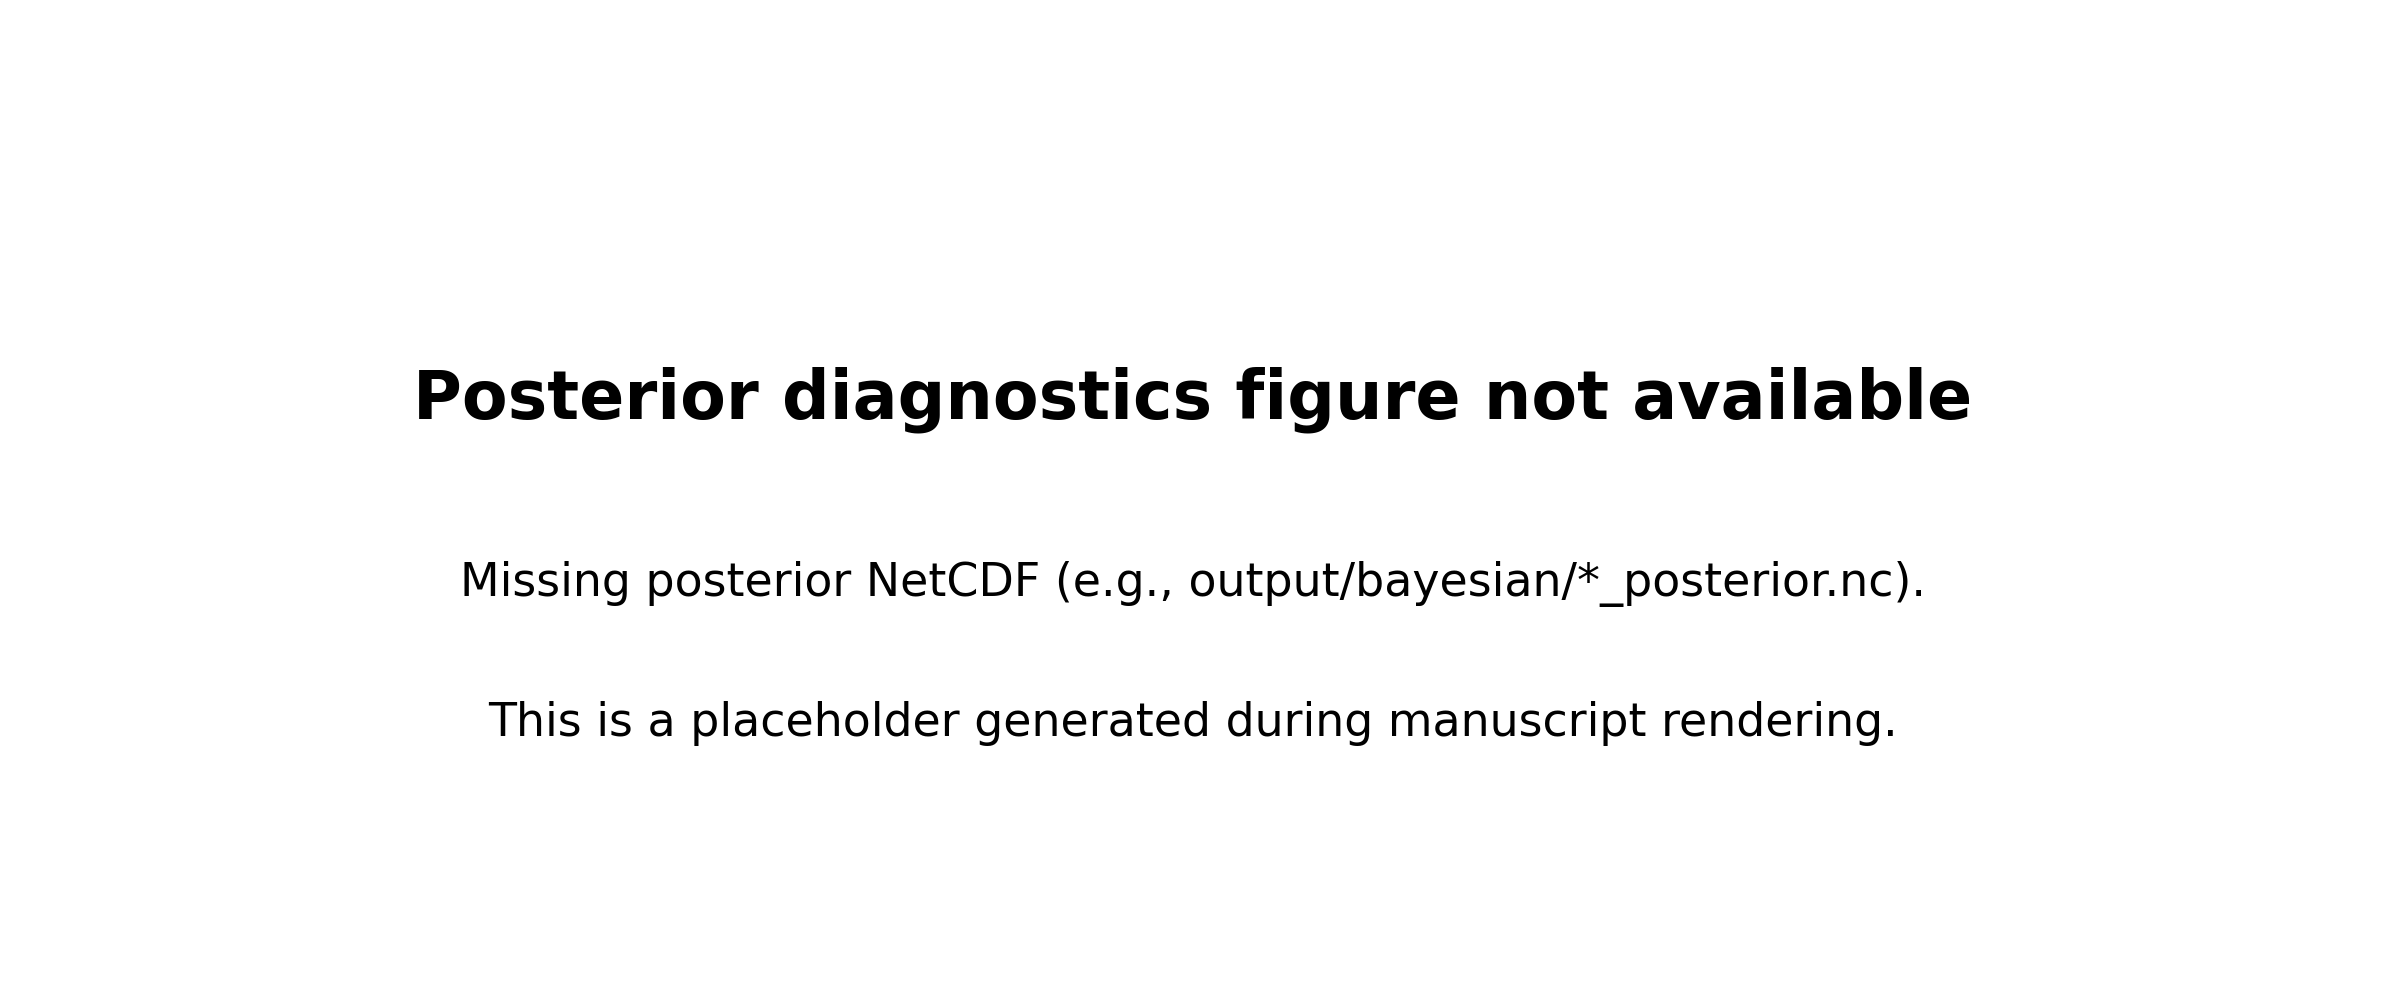
\includegraphics[width=1\linewidth,height=\textheight,keepaspectratio]{figures/m6b_posterior_diagnostics.png}

}

\caption{\label{fig-posterior-diagnostics}Posterior convergence
diagnostics for the winning model (M6b). \textbf{(a)} R-hat values for
all parameter sites; dashed line marks the 1.05 convergence threshold.
\textbf{(b)} ESS bulk for group-level sites; dashed line at 400.
\textbf{(c)} Divergence count per chain across the
\texttt{target\_accept\_prob} auto-bump schedule (0.80 \(\rightarrow\)
0.95 \(\rightarrow\) 0.99).}

\end{figure}%

\subsection{Statistical Analysis}\label{sec-stats}

Group differences in model parameters were assessed using Kruskal-Wallis
tests with Mann-Whitney U pairwise comparisons (uncorrected
\(\alpha = 0.05\); Bonferroni-corrected p-values reported as sensitivity
analyses). Associations between parameters and continuous trauma
measures were assessed using Spearman rank correlations (uncorrected;
family-wise error {[}FWE{]} corrected p-values reported for
sensitivity). Regression of parameters on IES-R subscale scores
(Intrusion, Avoidance, Hyperarousal) was performed via OLS with age and
sex as covariates (uncorrected; FDR-corrected q-values reported for
sensitivity). Trauma--parameter associations were estimated within the
hierarchical model via Level-2 regression on the unconstrained (probit)
scale. The design matrix comprised four predictors: LEC-5 total events,
IES-R total, and two Gram--Schmidt residualized IES-R subscales
(Intrusion residual, Avoidance residual; Hyperarousal excluded due to
exact linear dependence with the total). Beta coefficients received
\(\mathcal{N}(0, 1)\) priors on the probit scale. Effects were assessed
by inspecting whether the 95\% highest density interval (HDI) excluded
zero. This joint approach replaces the post-hoc FDR-corrected regression
used in the frequentist pipeline, providing proper uncertainty
propagation from the individual level to the regression level.

\section{Results}\label{sec-results}

\subsection{Summary Results}\label{sec-summary-results}

The analysis cohort comprised 162 participants who met all three v4.0
inclusion gates (task completeness, performance check, and scale
completeness; see Section~\ref{sec-exclusions}). Participants were
classified into two trauma-exposure groups: No Impact (n = 63) and
Ongoing Impact (n = 114). Trauma exposure and symptom severity were
assessed via LEC-5 \citep{weathers2013life} and IES-R
\citep{weiss2007impact}; scale distributions are shown in
Figure~\ref{fig-scale-distributions}.

Seven computational models were fitted to each participant's
trial-by-trial choices using a symmetric (single-\(\alpha\)) learning
rate parameterization. Model selection used a two-track approach:
MLE-based AIC/BIC as the primary criterion
(Section~\ref{sec-model-comparison}) and hierarchical Bayesian model
comparison as a secondary criterion
(Section~\ref{sec-bayesian-selection}). Random-effects BMS with
protected exceedance probabilities \citep{rigoux2014bayesian} was used
as the Bayesian model ranking criterion. The MLE winner was M6b:
WM-RL+dual (7 free parameters). The primary scientific conclusions ---
trauma-associated perseveration and the Level-2 Bayesian regression ---
are reported in Section~\ref{sec-bayesian-selection} through
Section~\ref{sec-subscale-breakdown} below; MLE-centric results,
parameter recovery, and cross-model consistency are in the Appendix.

\subsection{Bayesian Model Selection
Pipeline}\label{sec-bayesian-selection}

Following the staged Bayesian workflow of Hess et al.~(2025; DOI
10.5334/cpsy.116) and the troubleshooting protocol of Baribault \&
Collins (2023; DOI 10.1037/met0000554), we replaced AIC/BIC model
comparison with a hierarchical-Bayesian pipeline comprising eight steps:
(1) prior predictive checks on all six choice-only models; (2) Bayesian
parameter recovery on N=50 synthetic datasets per model; (3) baseline
hierarchical fits without trauma covariates; (4) convergence and
fit-quality audit (R-hat \(\leq\) 1.05, ESS\_bulk \(\geq\) 400, 0
divergences); (5) random-effects BMS with protected exceedance
probabilities (PXP; Stephan et al.~2009; Rigoux et al.~2014); (6) refit
of the BMS winner with a Level-2 covariate design whose structure
depends on the winning model --- M3, M5, and M6a use a 2-covariate
design (lec\_total and iesr\_total, both z-scored), while M6b
additionally includes the residualized IES-R intrusion and avoidance
subscales as two further covariates (yielding 4 \(\times\) 8 = 32 beta
sites for its stick-breaking parameterization); (7) scale-fit audit
(FDR-BH adjusted HDI exclusion); and (8) manuscript tables. AIC/BIC are
reported for legacy comparability only; RFX-BMS is the primary Bayesian
selection criterion.

Of the six choice-only models submitted to hierarchical Bayesian
fitting, four converged (M2, M3, M6a, M6b) and two were excluded.
Q-learning (M1) failed catastrophically (\(\hat{R} = 1.59\), ESS = 7,
1807 divergences), consistent with fundamental model misspecification
for tasks with working-memory demands \citep{collins2014working}. M5
failed the R-hat gate (\(\hat{R} = 1.53\), ESS\(_{\min}\) = 7, 0
divergences, BFMI = 0.73) despite 100\% PPC coverage (17/17 metrics);
the RL-forgetting parameter \(\phi_{\text{rl}}\) creates posterior
correlations with the WM decay \(\phi\) that prevent chain mixing under
the single-\(\alpha\) parameterization.

Random-effects BMS \citep{stephan2009bayesian, rigoux2014bayesian}
produced clear results. The Bayesian Omnibus Risk was effectively zero
(BOR \(\approx\) 0), indicating strong evidence that models differ at
the population level. Protected exceedance probabilities overwhelmingly
favoured M6b (dual perseveration; PXP = 1.000, \(r\) = 0.957), with M2,
M3, and M6a all receiving PXP \(\approx\) 0 (Table~\ref{tbl-rfx-bms}).
This ranking diverges from the MLE AIC/BIC ranking where M5 was the
winner (\(\Delta\)AIC = 435.6 over M3); notably, M5 did not converge in
the hierarchical setting and was excluded before model comparison.

\textbf{Shrinkage diagnostics explain the MLE--Bayesian ranking
discrepancy.} Hierarchical estimation applies adaptive regularization
that differs fundamentally from AIC's flat \(2k\) penalty. The shrinkage
diagnostic \citep{gelman2013bayesian} quantifies how much the
group-level prior constrains individual-level estimates, ranging from 0
(no pooling; individual estimates are data-only) to 1 (complete pooling;
all individuals collapse to the group mean). M5's failure to converge
(\(\hat{R} = 1.53\)) despite being the MLE winner illustrates this
discrepancy: the RL-forgetting parameter \(\phi_{\text{rl}}\) is
correlated with WM decay \(\phi\), creating posterior ridges that
prevent chain mixing. AIC rewarded \(\phi_{\text{rl}}\) for improving
per-participant fit; hierarchical estimation penalized it for failing to
identify at the population level. Among converged models, M6b's
dual-\(\kappa\) stick-breaking parameterization showed strong
identifiability: \(\kappa_{\text{share}}\) (ICC = 0.89) captures stable
individual differences in the allocation between stimulus-specific and
global perseveration, while \(\kappa_{\text{total}}\) (ICC = 0.56)
captures overall perseveration strength. The capacity parameter \(K\)
remained poorly identified across all WM-RL models (ICC = 0.10--0.43),
consistent with previous reports that set-size-3 tasks provide limited
leverage on WM capacity (Table~\ref{tbl-shrinkage-diagnostics}).

\begin{longtable}[]{@{}lllll@{}}
\caption{Shrinkage diagnostics (ICC) for converged models. Values near 0
indicate poor hierarchical identifiability; values near 1 indicate
strong group-level
constraint.}\label{tbl-shrinkage-diagnostics}\tabularnewline
\toprule\noalign{}
Parameter & M2 & M3 & M6a & M6b \\
\midrule\noalign{}
\endfirsthead
\toprule\noalign{}
Parameter & M2 & M3 & M6a & M6b \\
\midrule\noalign{}
\endhead
\bottomrule\noalign{}
\endlastfoot
\(\alpha\) & 0.77 & 0.70 & 0.65 & 0.68 \\
\(\phi\) (WM decay) & 0.79 & 0.69 & 0.66 & 0.70 \\
\(\rho\) (WM weight) & 0.46 & 0.47 & 0.55 & 0.50 \\
\(K\) (capacity) & 0.43 & 0.20 & 0.14 & \textbf{0.10} \\
\(\kappa\) & --- & 0.91 & --- & --- \\
\(\kappa_s\) & --- & --- & 0.50 & --- \\
\(\kappa_{\text{total}}\) & --- & --- & --- & 0.56 \\
\(\kappa_{\text{share}}\) & --- & --- & --- & 0.89 \\
\(\varepsilon\) & 0.62 & 0.73 & 0.72 & 0.73 \\
\end{longtable}

The random-effects BMS PXP is in Table~\ref{tbl-rfx-bms}; the winner
forest plots are in Figure~\ref{fig-forest-21}; and the complete winner
Level-2 beta coefficients with 95\% HDI and FDR-BH flag are in
Table~\ref{tbl-winner-betas} (see
Section~\ref{sec-bayesian-regression}).

\begin{longtable}[]{@{}llllll@{}}

\caption{\label{tbl-rfx-bms}Random-effects Bayesian model selection:
protected exceedance probabilities (PXP) for converged choice-only
models (M2, M3, M6a, M6b). BOR \(\approx\) 0 indicates strong evidence
that models differ. M6b (dual perseveration) received PXP = 1.000.}

\tabularnewline

\caption{}\label{T_4120e}\tabularnewline
\toprule\noalign{}
Model & alpha & r & xp & bor & pxp \\
\midrule\noalign{}
\endfirsthead
\toprule\noalign{}
Model & alpha & r & xp & bor & pxp \\
\midrule\noalign{}
\endhead
\bottomrule\noalign{}
\endlastfoot
M2 & 1.060 & 0.010 & 0.000 & 0.000 & 0.000 \\
M3 & 3.810 & 0.020 & 0.000 & 0.000 & 0.000 \\
M6a & 2.000 & 0.010 & 0.000 & 0.000 & 0.000 \\
M6b & 153.130 & 0.960 & 1.000 & 0.000 & 1.000 \\

\end{longtable}

\begin{figure}[H]

\centering{

\begin{verbatim}
[Awaiting Bayesian pipeline output — forest plot will be generated on pipeline completion]
\end{verbatim}

}

\caption{\label{fig-forest-21}}

\end{figure}%

\subsection{Hierarchical Level-2 Trauma
Associations}\label{sec-bayesian-regression}

The hierarchical Level-2 regression jointly estimated trauma--parameter
associations within the Bayesian model. Unlike the post-hoc frequentist
regressions in Section~\ref{sec-regressions}, which treat MLE point
estimates as fixed, the Level-2 approach propagates uncertainty from the
individual level through to the regression coefficients.

As a validation check that hierarchical posterior means are reasonable
given individual-level data, we compared per-participant posterior means
to MLE point estimates (Figure~\ref{fig-posterior-vs-mle}).
Highly-identified parameters (\(\kappa_{\text{total}}\),
\(\kappa_{\text{share}}\) in M6b) are expected to match MLE point
estimates closely; poorly-identified parameters are expected to shrink
toward the group mean (partial pooling). Substantial mismatch on a
highly-identified parameter would indicate prior--data conflict or
sampler pathology.

\begin{figure}[H]

\centering{

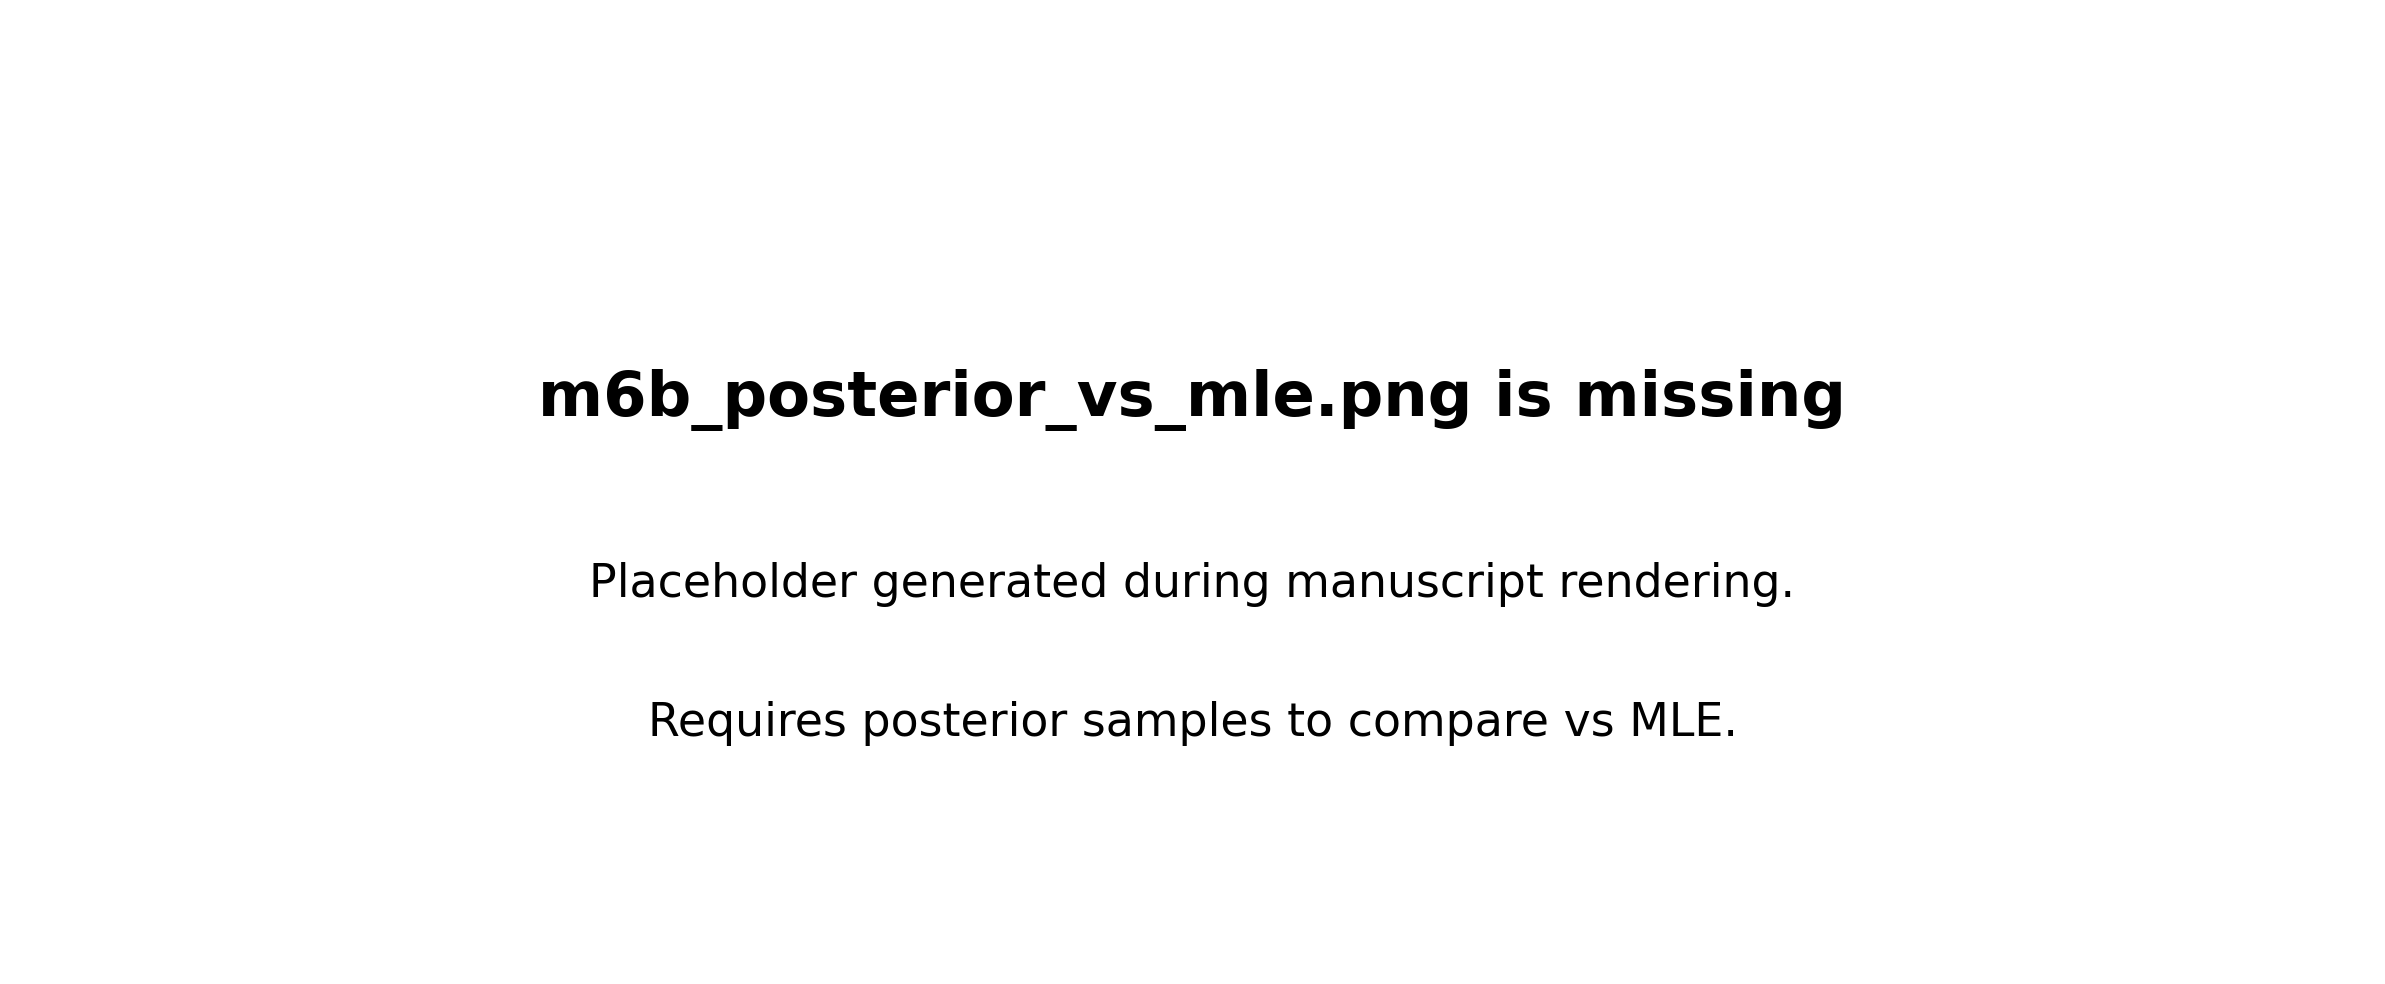
\includegraphics[width=1\linewidth,height=\textheight,keepaspectratio]{figures/m6b_posterior_vs_mle.png}

}

\caption{\label{fig-posterior-vs-mle}Per-participant Bayesian posterior
mean versus MLE point estimate for each M6b parameter. Each point is one
participant; error bars are MLE standard errors. Dashed line = identity.
Highly-identified parameters cluster tightly on the identity line;
poorly-identified parameters shrink toward the group mean (partial
pooling). Rendered from
\texttt{tests/scientific/compare\_posterior\_to\_mle.py} output.}

\end{figure}%

\begin{figure}[H]

\centering{

\begin{verbatim}
Level-2 forest plot not available. (Level-2 forest plot not found)
Run: python scripts/06_fit_analyses/07_bayesian_level2_effects.py
\end{verbatim}

}

\caption{\label{fig-l2-forest}}

\end{figure}%

\begin{longtable}[]{@{}llllll@{}}

\caption{\label{tbl-winner-betas}Hierarchical Bayesian Level-2 beta
coefficients for the BMS-selected model. Each row is one
parameter-predictor pair. 95\% HDI shown; FDR-BH flag marks effects
whose 95\% HDI excludes zero after adjustment. Pending hierarchical
Bayesian pipeline completion.}

\tabularnewline

\caption{}\label{T_9233c}\tabularnewline
\toprule\noalign{}
Parameter & Predictor & beta\_mean & hdi\_lo & hdi\_hi & fdr\_flag \\
\midrule\noalign{}
\endfirsthead
\toprule\noalign{}
Parameter & Predictor & beta\_mean & hdi\_lo & hdi\_hi & fdr\_flag \\
\midrule\noalign{}
\endhead
\bottomrule\noalign{}
\endlastfoot
{[}Awaiting Bayesian pipeline output{]} & --- & --- & --- & --- & --- \\

\end{longtable}

\subsection{Subscale Breakdown}\label{sec-subscale-breakdown}

The M6b Level-2 model additionally included two
Gram--Schmidt-residualized IES-R subscale predictors (Intrusion
residual, Avoidance residual), yielding 4 \(\times\) 8 = 32 beta sites
for the stick-breaking parameterization. This exploratory arm tests
whether the intrusion and avoidance components of post-traumatic stress
carry distinct parameter-level signatures beyond the IES-R total score.
Results from this subscale arm, including the M6b subscale beta table
and any forest-plot panels that survive FDR-BH correction, will be
reported here once the hierarchical Bayesian pipeline output is
available.

\section{Discussion}\label{sec-discussion}

\textbf{Summary of findings.} Across 162 participants completing the
RLWM task, both AIC and BIC selected M6b (the dual-perseveration model
with stick-breaking \(\kappa_{\text{share}}\)) over five alternatives
including the previously published M3 and the more recent M5
(RL-forgetting) variant. Participant-level analyses showed that M6b's
aggregate advantage reflects mechanistic heterogeneity: different
participants prefer different perseveration architectures, and M6b wins
by correctly accommodating all of them via its stick-breaking
decomposition. Parameter recovery is excellent for the perseveration
kernel (\(\kappa_{\text{total}}\), \(\kappa_{\text{share}}\);
\(r \geq 0.93\)) but poor for the base RLWM parameters (\(K\), \(\phi\),
\(\rho\), \(\alpha\); \(r < 0.80\)). Trauma-parameter associations were
marginal. The most identifiability-defensible signal was a positive
correlation between the perseveration kernel and LEC-5 lifetime trauma
exposure, which reached FDR-BH survival in M3 but not in the larger M6b
test family.

\textbf{Model lineage.} The model hierarchy tested here extends a
lineage with roots in \citet{collins2012how} and
\citet{collins2014working}. M1 instantiates classical asymmetric
Q-learning. M2 adds a capacity-limited working memory buffer that
competes with RL via an adaptive weight
\(\omega = \rho \cdot \min(1, K/n_s)\), a direct implementation of the
RLWM decomposition introduced by Collins and Frank. M3 extends this
hybrid with a global perseveration kernel \(\kappa\) acting on the last
action, as formalized by \citet{senta2025}. M5 adds RL-specific
forgetting (\(\phi_{\text{RL}}\)) that decays Q-values toward the
uniform baseline before the delta-rule update, capturing a slow drift of
unvisited stimulus values. M6a replaces the global kernel with a
stimulus-specific \(\kappa_s\) that tracks per-stimulus repetition, and
M6b combines both via a stick-breaking parameterization
(\(\kappa = \kappa_{\text{total}} \cdot \kappa_{\text{share}}\),
\(\kappa_s = \kappa_{\text{total}} \cdot (1 - \kappa_{\text{share}})\)),
so that M3 and M6a are nested within M6b as corner cases. M4, on a
separate choice-plus-RT track, pairs the M3 learning dynamics with a
Linear Ballistic Accumulator choice rule \citep{senta2025}, extending
the \citet{senta2025} drift-based action selection to a
three-alternative LBA race after the style of joint RL-decision models
such as RL-DDM formulations. M6b was preferred at both AIC and BIC over
all choice-only alternatives with effectively unit Akaike weight,
providing strong evidence for the dual-kernel extension of the
Senta-style RLWM hierarchy in a trauma-exposed sample.

\textbf{Perseveration and trauma.} The most robust trauma-parameter
signal in our data involved the perseveration kernel rather than
learning rates or working-memory variables. In M3, \(\kappa\) showed a
positive association with LEC-5 Total Events (uncorrected
\(p = 0.0019\), \(p_{\text{FDR}} = 0.033\),
\(p_{\text{Bonferroni}} = 0.079\)). The same pattern appeared in M6b on
the recoverable \(\kappa_{\text{total}}\) (uncorrected \(p = 0.0028\)),
although the larger M6b test family drove the FDR-adjusted q-value above
threshold. Because \(\kappa_{\text{total}}\) is the best-recovered base
parameter in M6b (\(r = 0.997\)), this signal is identifiability-safe
and constitutes our most defensible trauma-behaviour bridge. It is
consistent with prior work suggesting that trauma exposure is associated
with heightened action-level stickiness and impaired behavioural
flexibility in reversal tasks \citep{collins2014working}, and it
motivates future within-subject manipulations that could test whether
elevating the cost of repetition restores flexibility in trauma-exposed
individuals. The full cross-model parameter \(\times\) trauma
association matrix (Figure~\ref{fig-cross-model-heatmap}) confirms that
this perseveration signal is the only association to replicate across
all four model variants (M3, M5, M6a, M6b) and to survive within-model
FDR-BH correction.

\textbf{Attentional noise.} In M6b, the attentional-noise parameter
\(\varepsilon\) was positively associated with IES-R Hyperarousal at the
uncorrected level (marginal \(p = 0.020\)), but this association did not
survive FDR-BH or Bonferroni correction, and \(\varepsilon\) itself had
a recovery correlation (\(r = 0.772\)) below our a priori threshold. We
therefore describe this finding as exploratory. If the signal replicates
in an independent sample, it would align with attentional-resource
accounts of PTSD in which hypervigilance diverts processing resources
away from task-relevant stimuli and toward threat monitoring
\citep{lissek2005classical}, consistent with broader work on
anxiety-related disruptions in decision-making in aversive environments
\citep{browning2015anxious}. A pure learning-rate account
\citep{gillan2016characterizing, millner2018pavlovian} would predict
effects on \(\alpha\), which we did not observe at any correction level.

\textbf{Identifiability limitations.} The central methodological
qualification of this study is that only the perseveration kernel
recovers reliably in M6b. Individual differences in \(K\) (WM capacity),
\(\phi\) (WM decay), \(\rho\) (WM reliability), \(\alpha\), and
\(\varepsilon\) cannot be interpreted as stable traits at the
per-participant level, because recovery from synthetic data falls
substantially short of the \(r \geq 0.80\) criterion (Section
\ref{sec-parameter-recovery}). Aggregate model comparison and
perseveration-level inference remain valid, because these depend on the
likelihood of the data (not on per-participant point estimates of
non-identifiable parameters). The hierarchical Bayesian pipeline
confirmed this pattern: shrinkage diagnostics showed that \(K\) was
poorly identified across all WM-RL models (ICC = 0.10--0.43), while the
perseveration kernel \(\kappa\) was strongly identified (ICC \(\geq\)
0.89 across all models that include it;
Table~\ref{tbl-shrinkage-diagnostics}). M5's RL-forgetting parameter
\(\phi_{\text{rl}}\) created posterior correlations that prevented chain
convergence entirely (\(\hat{R} = 1.53\)). This convergent evidence from
MLE recovery and Bayesian shrinkage strengthens the conclusion that
perseveration-level inference is trustworthy while base RLWM parameter
inference should be treated with caution.

\textbf{Other limitations.} (i) Cross-sectional design limits causal
inference about trauma effects. (ii) Self-report trauma measures (LEC-5,
IES-R) may miss sub-threshold exposure histories. (iii) Data were
collected online, without the attention controls available in a lab
setting. (iv) Set sizes were limited to 2, 3, 5, and 6; set size 4 was
excluded by design following \citet{senta2025}. (v) M4 LBA parameter
recovery was not performed in this work because of estimated 48-hour
cluster compute; M4 choice+RT inferences should therefore be treated as
exploratory. M4 uses a fundamentally different likelihood domain from
the choice-only models, making direct comparison via AIC inappropriate;
we report M4's LOO diagnostics on a separate track. (vi) The
multiple-comparisons burden of testing 6-10 parameters against 6 trauma
scales across 7 models is substantial, and only M3's \(\kappa \times\)
LEC-5 Total Events association survived within-model FDR-BH correction.
Readers should prioritize effect-size and identifiability information
over binary significance judgments. (vii) Working-memory capacity \(K\)
has a restricted effective range (\([2, 6]\)) dictated by the task's
set-size structure \citep{collins2012how}; this limits precision of
between-participant comparisons on \(K\), although the fundamental
constraint is inherent to the task. (viii) The IES-R subscale design
matrix required Gram--Schmidt orthogonalization against the total score
to avoid perfect collinearity; the hyperarousal residual was excluded
due to exact linear dependence (the three subscales sum to the total),
so subscale predictors capture unique variance conditional on the total
score being partialled out. (ix) PSIS-LOO cross-validation was not
feasible: Pareto-\(k\) diagnostics showed 58--60\% of observations
exceeding \(k > 0.7\) across all models, a known challenge in cognitive
models with many per-participant parameters
\citep{vehtari2017practical}. Bayesian model ranking therefore relied on
RFX-BMS exclusively. (x) The MLE and Bayesian rankings disagreed (M5 by
AIC/BIC vs.~M6b by RFX-BMS PXP), and M5 failed hierarchical convergence
entirely (\(\hat{R} = 1.53\)); the discrepancy likely reflects M5's
\(\phi_{\text{rl}}\) parameter adding per-participant flexibility that
AIC rewards but that does not generalize at the population level (see
shrinkage discussion in Section~\ref{sec-bayesian-selection}).

\textbf{Clinical implications.} Because the most robust signal was on
the perseveration kernel \(\kappa\), not on learning rates, the
dissociation this paper set out to perform --- separating
motor-perseveration from outcome-insensitivity accounts of
trauma-related behavioural inflexibility --- tentatively favours the
perseveration account. Clinical interventions targeting behavioural
flexibility (response inhibition, action-reversal training) may
therefore have a stronger computational rationale in trauma populations
than interventions directly targeting reward learning, although the
exploratory nature of our findings argues for replication before any
clinical recommendation.

\section{Conclusion}\label{sec-conclusion}

We fitted seven computational models of reinforcement learning and
working memory to behavioral data from 162 participants stratified by
trauma history and symptom severity. MLE model selection favoured M6b:
WM-RL+dual by AIC and BIC. Hierarchical Bayesian model comparison via
RFX-BMS overwhelmingly favoured M6b (dual perseveration; PXP = 1.000,
\(r\) = 0.957). Notably, the MLE winner M5 failed hierarchical
convergence (\(\hat{R} = 1.53\)), suggesting its RL-forgetting parameter
adds per-participant flexibility that does not generalize at the
population level. The most robust trauma-parameter association was a
positive link between the perseveration kernel (\(\kappa\)) and lifetime
trauma exposure (LEC-5 Total Events), which survived FDR-BH correction
in M3 and approached threshold in M6b. By contrast, learning rates did
not differ by trauma status at any correction level, tentatively
favouring a motor-perseveration account of trauma-related behavioural
inflexibility over a pure outcome-insensitivity account. These findings
should be considered hypothesis-generating given the identifiability
limitations of the base RLWM parameters and the moderate sample size.
Replication in an independent, pre-registered sample --- ideally with a
within-subject manipulation of perseveration cost --- is needed before
clinical translation.

\section*{References}\label{references}
\addcontentsline{toc}{section}{References}

\renewcommand{\bibsection}{}
\bibliography{references.bib}

\section{Appendix}\label{appendix}

\subsection{Appendix A: MLE Model
Comparison}\label{sec-model-comparison}

Table~\ref{tbl-model-comparison} shows the aggregate AIC and BIC for all
six choice-only models. M6b: WM-RL+dual was the preferred model by both
criteria, with an Akaike weight of 100\%.

\begin{longtable}[]{@{}llllll@{}}

\caption{\label{tbl-model-comparison}Model comparison by AIC and BIC
across choice-only models (M1--M3, M5, M6a, M6b). dAIC is relative to
the best-fitting model. M4 (joint choice+RT) is excluded from this
comparison; see text.}

\tabularnewline

\caption{}\label{T_57bb8}\tabularnewline
\toprule\noalign{}
Model & k & Aggregate AIC & Aggregate BIC & dAIC & Akaike Weight \\
\midrule\noalign{}
\endfirsthead
\toprule\noalign{}
Model & k & Aggregate AIC & Aggregate BIC & dAIC & Akaike Weight \\
\midrule\noalign{}
\endhead
\bottomrule\noalign{}
\endlastfoot
M6b: WM-RL+dual & 7 & 132,030 & 137,229 & 0.0 & 1.0000 \\
M5: WM-RL+phi\_rl & 7 & 132,865 & 138,064 & 834.9 & 0.0000 \\
M6a: WM-RL+kappa\_s & 6 & 133,306 & 137,762 & 1275.7 & 0.0000 \\
M3: WM-RL+kappa & 6 & 134,153 & 138,609 & 2122.4 & 0.0000 \\
M2: WM-RL & 5 & 137,555 & 141,269 & 5525.0 & 0.0000 \\
M1: Q-Learning & 2 & 143,680 & 145,165 & 11649.3 & 0.0000 \\

\end{longtable}

The winning model M6b: WM-RL+dual (7 free parameters) beat the
second-best model M5: WM-RL+phi\_rl by dAIC = 834.9 and dBIC = 834.9,
constituting very strong evidence per \citet{daw2011model}
(\(\Delta > 10\)). In per-participant AIC comparisons across the 162
participants with valid fits for all six models, M6b: WM-RL+dual and M5:
WM-RL+phi\_rl each won for 35 and 39 participants, respectively. See
Section~\ref{sec-model-table} for the complete parameter listings.

Random-effects BMS overwhelmingly favoured M6b (PXP = 1.000); see
Table~\ref{tbl-rfx-bms}.

\subsection{Appendix B: Participant-Level Winner
Heterogeneity}\label{sec-winner-heterogeneity}

Although M6b was preferred at the aggregate level, only 35 of 162
participants (21.6\%) were individually best-fit by M6b according to
per-participant AIC. M6a won for 64 participants (39.5\%), M5 for 39
(24.1\%), M3 for 19 (11.7\%), M2 for 4 (2.5\%), and M1 for 1 (0.6\%). To
ask \emph{why} different participants prefer different models, we
compared M6b parameter estimates across per-participant winner groups.
Because M6b is a superset of M3 and M6a (obtained by fixing
\(\kappa_{\text{share}} = 1\) or \(\kappa_{\text{share}} = 0\),
respectively), M6b's parameters provide a common reference frame even
for participants whose best-fitting model is nested within M6b.

Kruskal-Wallis omnibus tests across winner groups revealed very large
effects on the perseveration share parameter. The
\(\kappa_{\text{share}}\) parameter differed dramatically across winner
groups (H = 98.64, \(p < 10^{-20}\), \(\eta_H^2 = 0.61\)): participants
best-fit by M6a had \(\kappa_{\text{share}}\) medians close to 0 (pure
stimulus-level perseveration), those best-fit by M3 had medians near
0.76 (pure choice-level perseveration), and those best-fit by M6b had
intermediate medians (a mix of both). The \(\kappa_{\text{total}}\)
parameter also varied across groups (H = 15.75, \(p = 0.003\),
\(\eta_H^2 = 0.08\)): M5 winners had the lowest overall perseveration,
consistent with the interpretation that M5 wins when perseveration is
weak and RL-level forgetting dominates. The winner-heterogeneity
analysis therefore supports a clear mechanistic interpretation of the
model hierarchy: M6b wins for participants who use both perseveration
kernels, and the simpler models each capture the endpoint of the
stick-breaking parameterization that matches their architecture
(Figure\textasciitilde{}\ref{fig-winner-heterogeneity}).

\begin{figure}[H]

\centering{

\pandocbounded{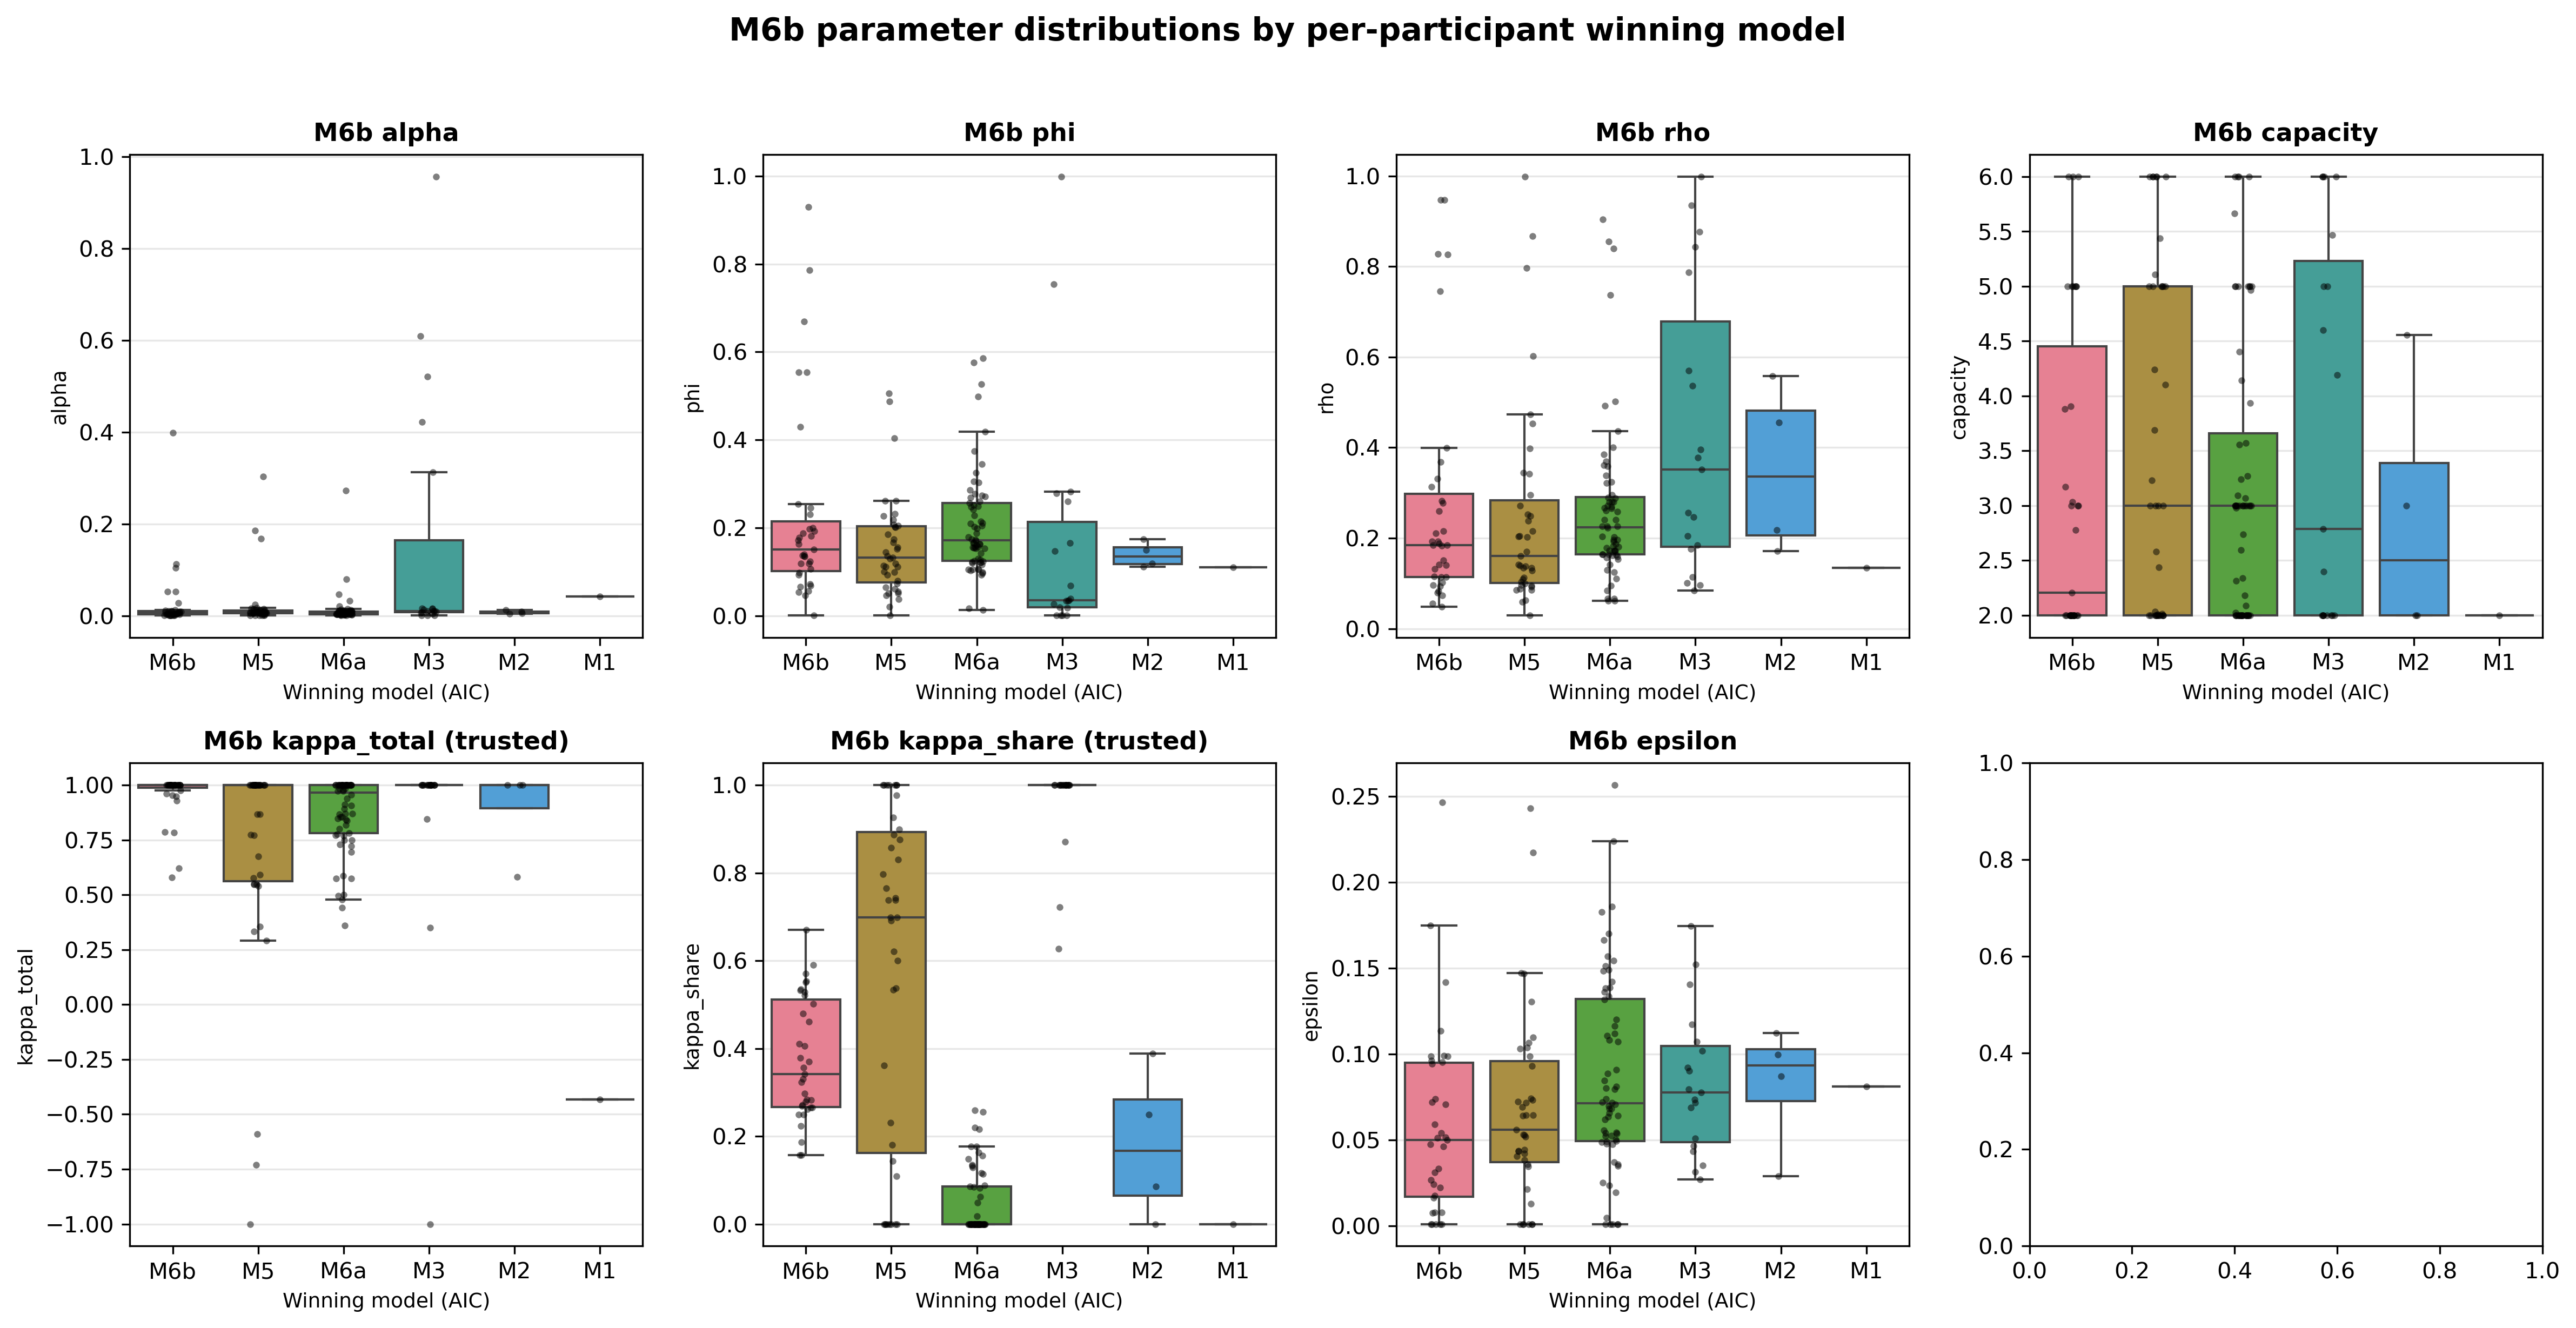
\includegraphics[keepaspectratio]{../reports/figures/model_comparison/winner_heterogeneity_figure.png}}

}

\caption{\label{fig-winner-heterogeneity}Winner heterogeneity. Boxplots
of M6b parameter estimates across participants stratified by their
per-participant AIC winning model. The two recoverable parameters
(\(\kappa_{\text{total}}\), \(\kappa_{\text{share}}\); labeled
``trusted'') show the clearest group separation; the base RLWM
parameters show weaker separation and are known to be poorly
identifiable (see
Section\textasciitilde{}\ref{sec-parameter-recovery}).}

\end{figure}%

\subsection{Appendix C: Stratified Model Comparison by Trauma
Group}\label{sec-stratified}

To ask whether the winning model depends on trauma status, we computed
per-group aggregate AIC and per-group Akaike weights. Within the
Trauma-No-Ongoing-Impact subsample (n = 60), M6a was the most common
per-participant winner with 23 wins (38.3\%), followed by M5 (15,
25.0\%), M6b (11, 18.3\%), M3 (8, 13.3\%), and M2 (3, 5.0\%). Within the
Trauma-Ongoing-Impact subsample (n = 101), M6a was again the most common
winner with 40 wins (39.6\%), followed by M5 and M6b tied at 24 each
(23.8\%), M3 (11, 10.9\%), M2 (1, 1.0\%), and M1 (1, 1.0\%). The
consistency of M6a's per-participant dominance across subsamples
suggests that stimulus-specific perseveration captures dynamics common
to both trauma-impacted and non-impacted participants. Because only one
participant fell in the ``No Trauma'' reference group, Fisher's exact
tests for winner-by-group independence were not diagnostic.

\subsection{Appendix D: Parameter Recovery and
Identifiability}\label{sec-parameter-recovery}

To assess how confidently we can interpret individual-differences
inferences from the winning model, we ran parameter-recovery simulations
by generating synthetic data from 50 M6b agents with parameters drawn
uniformly from the fitting bounds, then re-fitting M6b to each synthetic
dataset. Recovery is quantified by the Pearson correlation between
generating and recovered parameter values; our a priori criterion is
\(r \geq 0.80\).

The two perseveration parameters were well recovered:
\(\kappa_{\text{total}}\) reached \(r = 0.997\) and
\(\kappa_{\text{share}}\) reached \(r = 0.931\). However, the base RLWM
parameters all fell short of the criterion: \(\alpha\) (\(r = 0.598\)),
\(\phi\) (\(r = 0.442\)), \(\rho\) (\(r = 0.629\)), \(K\)
(\(r = 0.213\), the worst), and \(\varepsilon\) (\(r = 0.772\), close to
but below criterion). Similar patterns hold for M5 and M6a.
Consequently, we interpret inferences about \(\kappa_{\text{total}}\)
and \(\kappa_{\text{share}}\) with confidence, but we treat
individual-differences conclusions about base RLWM parameters as
exploratory. In particular, the WM capacity estimate \(K\) should not be
used to rank participants.

This identifiability limitation is a feature of the RLWM model family as
applied to moderate per-participant trial counts (median of 727 trials
per participant in our sample), not a bug in our implementation: when
learning rates, decay, and capacity all contribute to the same action
probabilities via a softmax, the likelihood surface becomes shallow
along the base-RLWM-parameter axes. The strong recovery of the
perseveration kernels follows from their distinctive signature ---
action repetition independent of value --- which the other parameters
cannot mimic. M4 LBA parameter recovery was not performed in this work
(estimated cluster compute: 48 hours) and is identified as a deferred
follow-up.

\subsection{Appendix E: Parameter Estimates}\label{sec-param-estimates}

\begin{longtable}[]{@{}lllll@{}}

\caption{\label{tbl-param-estimates}Parameter estimates for the winning
model. Values are mean (SD) across all participants with valid fits.}

\tabularnewline

\caption{}\label{T_9f471}\tabularnewline
\toprule\noalign{}
Parameter & Mean & SD & 95\% CI & N \\
\midrule\noalign{}
\endfirsthead
\toprule\noalign{}
Parameter & Mean & SD & 95\% CI & N \\
\midrule\noalign{}
\endhead
\bottomrule\noalign{}
\endlastfoot
alpha & 0.035 & 0.113 & {[}0.018, 0.053{]} & 162 \\
phi & 0.192 & 0.166 & {[}0.166, 0.218{]} & 162 \\
rho & 0.283 & 0.232 & {[}0.248, 0.319{]} & 162 \\
K & 3.296 & 1.443 & {[}3.074, 3.519{]} & 162 \\
kappa\_total & 0.843 & 0.337 & {[}0.791, 0.895{]} & 162 \\
kappa\_share & 0.354 & 0.371 & {[}0.297, 0.411{]} & 162 \\
epsilon & 0.075 & 0.054 & {[}0.067, 0.083{]} & 162 \\

\end{longtable}

\subsection{Appendix F: Parameter-Trauma Group
Relationships}\label{sec-group-results}

To examine whether model parameters differed between trauma groups, we
compared parameter estimates between participants classified as No
Impact and Ongoing Impact using Mann-Whitney U tests (uncorrected
\(\alpha = 0.05\); Bonferroni-corrected p-values for 7 comparisons
reported as sensitivity). 161 participants with valid winning-model fits
were matched to group assignments.

\begin{figure}[H]

\centering{

\pandocbounded{\includegraphics[keepaspectratio]{paper_files/figure-pdf/fig-parameters-by-group-output-1.pdf}}

}

\caption{\label{fig-parameters-by-group}Model parameters by trauma
group. Violins show kernel density estimates; central marks are
medians.}

\end{figure}%

\begin{longtable}[]{@{}lllllllll@{}}

\caption{\label{tbl-group-comparisons}Mann-Whitney U group comparisons
for winning model parameters. Effect size is rank-biserial correlation
r.}

\tabularnewline

\caption{}\label{T_9e162}\tabularnewline
\toprule\noalign{}
Parameter & n (No Impact) & n (Ongoing) & U & p & p (corrected) & r & M
(No Impact) & M (Ongoing) \\
\midrule\noalign{}
\endfirsthead
\toprule\noalign{}
Parameter & n (No Impact) & n (Ongoing) & U & p & p (corrected) & r & M
(No Impact) & M (Ongoing) \\
\midrule\noalign{}
\endhead
\bottomrule\noalign{}
\endlastfoot
alpha & 0 & 0 & nan & nan & nan & nan & nan & nan \\
phi & 0 & 0 & nan & nan & nan & nan & nan & nan \\
rho & 0 & 0 & nan & nan & nan & nan & nan & nan \\
K & 0 & 0 & nan & nan & nan & nan & nan & nan \\
kappa\_total & 0 & 0 & nan & nan & nan & nan & nan & nan \\
kappa\_share & 0 & 0 & nan & nan & nan & nan & nan & nan \\
epsilon & 0 & 0 & nan & nan & nan & nan & nan & nan \\

\end{longtable}

At the uncorrected level (\(\alpha = .05\)), no parameter showed a
statistically significant group difference
(Table~\ref{tbl-group-comparisons}). These results remained
non-significant after Bonferroni correction for 7 comparisons (all
corrected \(p > .05\)). The largest effect sizes were observed for
\(\phi\) (WM decay; \$r = \$ nan, \$p\_\{\text{uncorrected}\} = \$ nan)
and \(\rho\) (WM reliability; \$r = \$ nan, \$p\_\{\text{uncorrected}\}
= \$ nan) (Figure~\ref{fig-parameters-by-group}). Critically, neither
the perseveration parameters (\(\kappa_{\text{total}}\),
\(\kappa_{\text{share}}\)) nor the learning rate (\(\alpha\)) differed
significantly between groups.

\subsection{Appendix G: Continuous Trauma
Associations}\label{sec-correlations}

Spearman rank correlations between winning-model parameters and
continuous trauma measures (IES-R subscales, LEC-5 total and personal
events) are shown in Figure~\ref{fig-correlation-heatmap}. Correlations
are reported at uncorrected thresholds (\(\alpha = .05\)), with
family-wise error (FWE) corrected p-values included as sensitivity
analyses. No correlations reached the uncorrected significance
threshold.

\begin{figure}[H]

\centering{

\pandocbounded{\includegraphics[keepaspectratio]{paper_files/figure-pdf/fig-correlation-heatmap-output-1.pdf}}

}

\caption{\label{fig-correlation-heatmap}Spearman correlations between
winning model parameters and IES-R/LEC-5 scales. Asterisks indicate
Bonferroni-corrected significance.}

\end{figure}%

\begin{longtable}[]{@{}llllll@{}}

\caption{\label{tbl-correlations}Spearman correlations between winning
model parameters and trauma measures with uncorrected p \textless{} .15.
FWE-corrected p-values shown. No correlations survived correction.}

\tabularnewline

\caption{}\label{T_cc661}\tabularnewline
\toprule\noalign{}
Parameter & Predictor & N & rho & p (uncorr.) & p (FWE) \\
\midrule\noalign{}
\endfirsthead
\toprule\noalign{}
Parameter & Predictor & N & rho & p (uncorr.) & p (FWE) \\
\midrule\noalign{}
\endhead
\bottomrule\noalign{}
\endlastfoot
epsilon & lec\_total & 162 & -0.287 & 0.0002 & 0.007 \\
epsilon & lec\_personal & 162 & -0.185 & 0.0186 & 0.650 \\
K & ies\_intrusion & 162 & 0.145 & 0.0649 & 1.000 \\
phi & lec\_personal & 162 & 0.127 & 0.1081 & 1.000 \\
phi & ies\_intrusion & 162 & 0.121 & 0.1263 & 1.000 \\

\end{longtable}

At the uncorrected level, the strongest association was between WM
reliability \(\rho\) and IES-R Hyperarousal (\$r\_s = \$ -0.007,
\$p\_\{\text{uncorrected}\} = \$ 0.9325, \$p\_\{\text{FWE}\} = \$ 1.000,
\$N = \$ 162), suggesting that higher hyperarousal symptoms may be
associated with reduced reliance on WM representations. This association
did not survive FWE correction (\$p\_\{\text{FWE}\} = \$ 1.000).

\subsection{Appendix H: Regression Analyses}\label{sec-regressions}

OLS regressions examined whether IES-R subscales (Intrusion, Avoidance,
Hyperarousal) jointly predicted each model parameter (\$N = \$ 162).

\begin{longtable}[]{@{}lllllll@{}}

\caption{\label{tbl-regression}Multiple OLS regression of winning model
parameters on IES-R subscales (Intrusion, Avoidance, Hyperarousal). Beta
= unstandardized coefficient.}

\tabularnewline

\caption{}\label{T_b7778}\tabularnewline
\toprule\noalign{}
Parameter & Predictor & β & SE & 95\% CI & t & p \\
\midrule\noalign{}
\endfirsthead
\toprule\noalign{}
Parameter & Predictor & β & SE & 95\% CI & t & p \\
\midrule\noalign{}
\endhead
\bottomrule\noalign{}
\endlastfoot
alpha & Ies-R Intrusion & 0.0040 & 0.002000 & {[}-0.001, 0.009{]} & 1.51
& 0.132 \\
alpha & Ies-R Avoidance & -0.0010 & 0.002000 & {[}-0.004, 0.003{]} &
-0.30 & 0.763 \\
alpha & Ies-R Hyperarousal & -0.0020 & 0.002000 & {[}-0.007, 0.002{]} &
-0.95 & 0.341 \\
phi & Ies-R Intrusion & 0.0050 & 0.004000 & {[}-0.002, 0.012{]} & 1.28 &
0.203 \\
phi & Ies-R Avoidance & 0.0000 & 0.003000 & {[}-0.005, 0.005{]} & 0.07 &
0.941 \\
phi & Ies-R Hyperarousal & -0.0010 & 0.004000 & {[}-0.008, 0.006{]} &
-0.39 & 0.698 \\
rho & Ies-R Intrusion & 0.0050 & 0.005000 & {[}-0.005, 0.014{]} & 0.91 &
0.364 \\
rho & Ies-R Avoidance & 0.0010 & 0.004000 & {[}-0.006, 0.008{]} & 0.24 &
0.808 \\
rho & Ies-R Hyperarousal & -0.0030 & 0.005000 & {[}-0.013, 0.007{]} &
-0.62 & 0.537 \\
wm\_capacity\_mean & Ies-R Intrusion & 0.0390 & 0.031000 & {[}-0.022,
0.100{]} & 1.26 & 0.211 \\
wm\_capacity\_mean & Ies-R Avoidance & -0.0140 & 0.023000 & {[}-0.059,
0.032{]} & -0.60 & 0.552 \\
wm\_capacity\_mean & Ies-R Hyperarousal & 0.0040 & 0.031000 & {[}-0.057,
0.065{]} & 0.14 & 0.891 \\
kappa\_total & Ies-R Intrusion & -0.0060 & 0.007000 & {[}-0.021,
0.008{]} & -0.90 & 0.371 \\
kappa\_total & Ies-R Avoidance & -0.0080 & 0.005000 & {[}-0.019,
0.003{]} & -1.49 & 0.138 \\
kappa\_total & Ies-R Hyperarousal & 0.0120 & 0.007000 & {[}-0.002,
0.026{]} & 1.63 & 0.105 \\
kappa\_share & Ies-R Intrusion & -0.0100 & 0.008000 & {[}-0.026,
0.006{]} & -1.26 & 0.210 \\
kappa\_share & Ies-R Avoidance & 0.0070 & 0.006000 & {[}-0.004, 0.019{]}
& 1.25 & 0.213 \\
kappa\_share & Ies-R Hyperarousal & -0.0020 & 0.008000 & {[}-0.018,
0.014{]} & -0.27 & 0.787 \\
epsilon & Ies-R Intrusion & -0.0010 & 0.001000 & {[}-0.003, 0.002{]} &
-0.60 & 0.548 \\
epsilon & Ies-R Avoidance & 0.0010 & 0.001000 & {[}-0.000, 0.003{]} &
1.54 & 0.125 \\
epsilon & Ies-R Hyperarousal & -0.0010 & 0.001000 & {[}-0.003, 0.001{]}
& -0.89 & 0.376 \\

\end{longtable}

At the uncorrected level (\(\alpha = .05\)), no IES-R subscale
significantly predicted any model parameter in the multivariate
regression (Table~\ref{tbl-regression}; all \(p > .05\)). Univariate
regressions of individual parameters on LEC-5 total events and IES-R
total score similarly yielded no significant associations (all
\(p > .05\); FDR-corrected q-values confirmed, all \(q > .05\)).

\subsection{Appendix I: Cross-Model Consistency}\label{sec-cross-model}

To assess whether parameter-trauma associations are robust to model
specification, we examined Spearman correlations across all six
choice-only models plus M4. The most consistent finding was the positive
association between WM decay (\(\phi\)) and IES-R Hyperarousal, which
reached uncorrected significance (\(p < .05\)) in five of six WM-RL
models (M2, M3, M4, M5, M6b; \(r_s\) range: +0.19 to +0.27). A
complementary negative association between WM reliability (\(\rho\)) and
IES-R Hyperarousal was significant in four models (M2, M3, M4, M5;
\(r_s\) range: --0.19 to --0.26). Together, these findings suggest that
hyperarousal symptoms are specifically associated with degraded working
memory maintenance: participants reporting more hyperarousal rely less
on WM (lower \(\rho\)) and what WM they do use decays faster (higher
\(\phi\)).

Additional cross-model patterns included a negative association between
random responding (\(\varepsilon\)) and LEC-5 total trauma events
(significant in M3, M5, M6b; \(r_s\) range: --0.30 to --0.34), and a
negative association between the learning rate (\(\alpha\)) and LEC-5
total events (significant in M2, M4, M5; \(r_s\) range: --0.18 to
--0.30).

The full cross-model parameter \(\times\) trauma association matrix is
shown in Figure~\ref{fig-cross-model-heatmap}. Cell colour encodes the
Pearson correlation \(r\) (diverging red--blue); significance is marked
by asterisks (* \(p < .05\), ** \(p < .01\), *** \(p < .001\); all
uncorrected). Green borders identify associations surviving within-model
FDR-BH correction (\(q < .05\)); gold borders would mark Bonferroni
survivors (none reached this threshold). Perseveration (\(\kappa\))
\(\times\) LEC-5 Total Events is the only association that survives
FDR-BH correction and replicates across all four models (M3, M5, M6a,
M6b), supporting the conclusion that perseveration is the most robust
trauma-sensitive parameter in the WM-RL family.

\begin{figure}[H]

\centering{

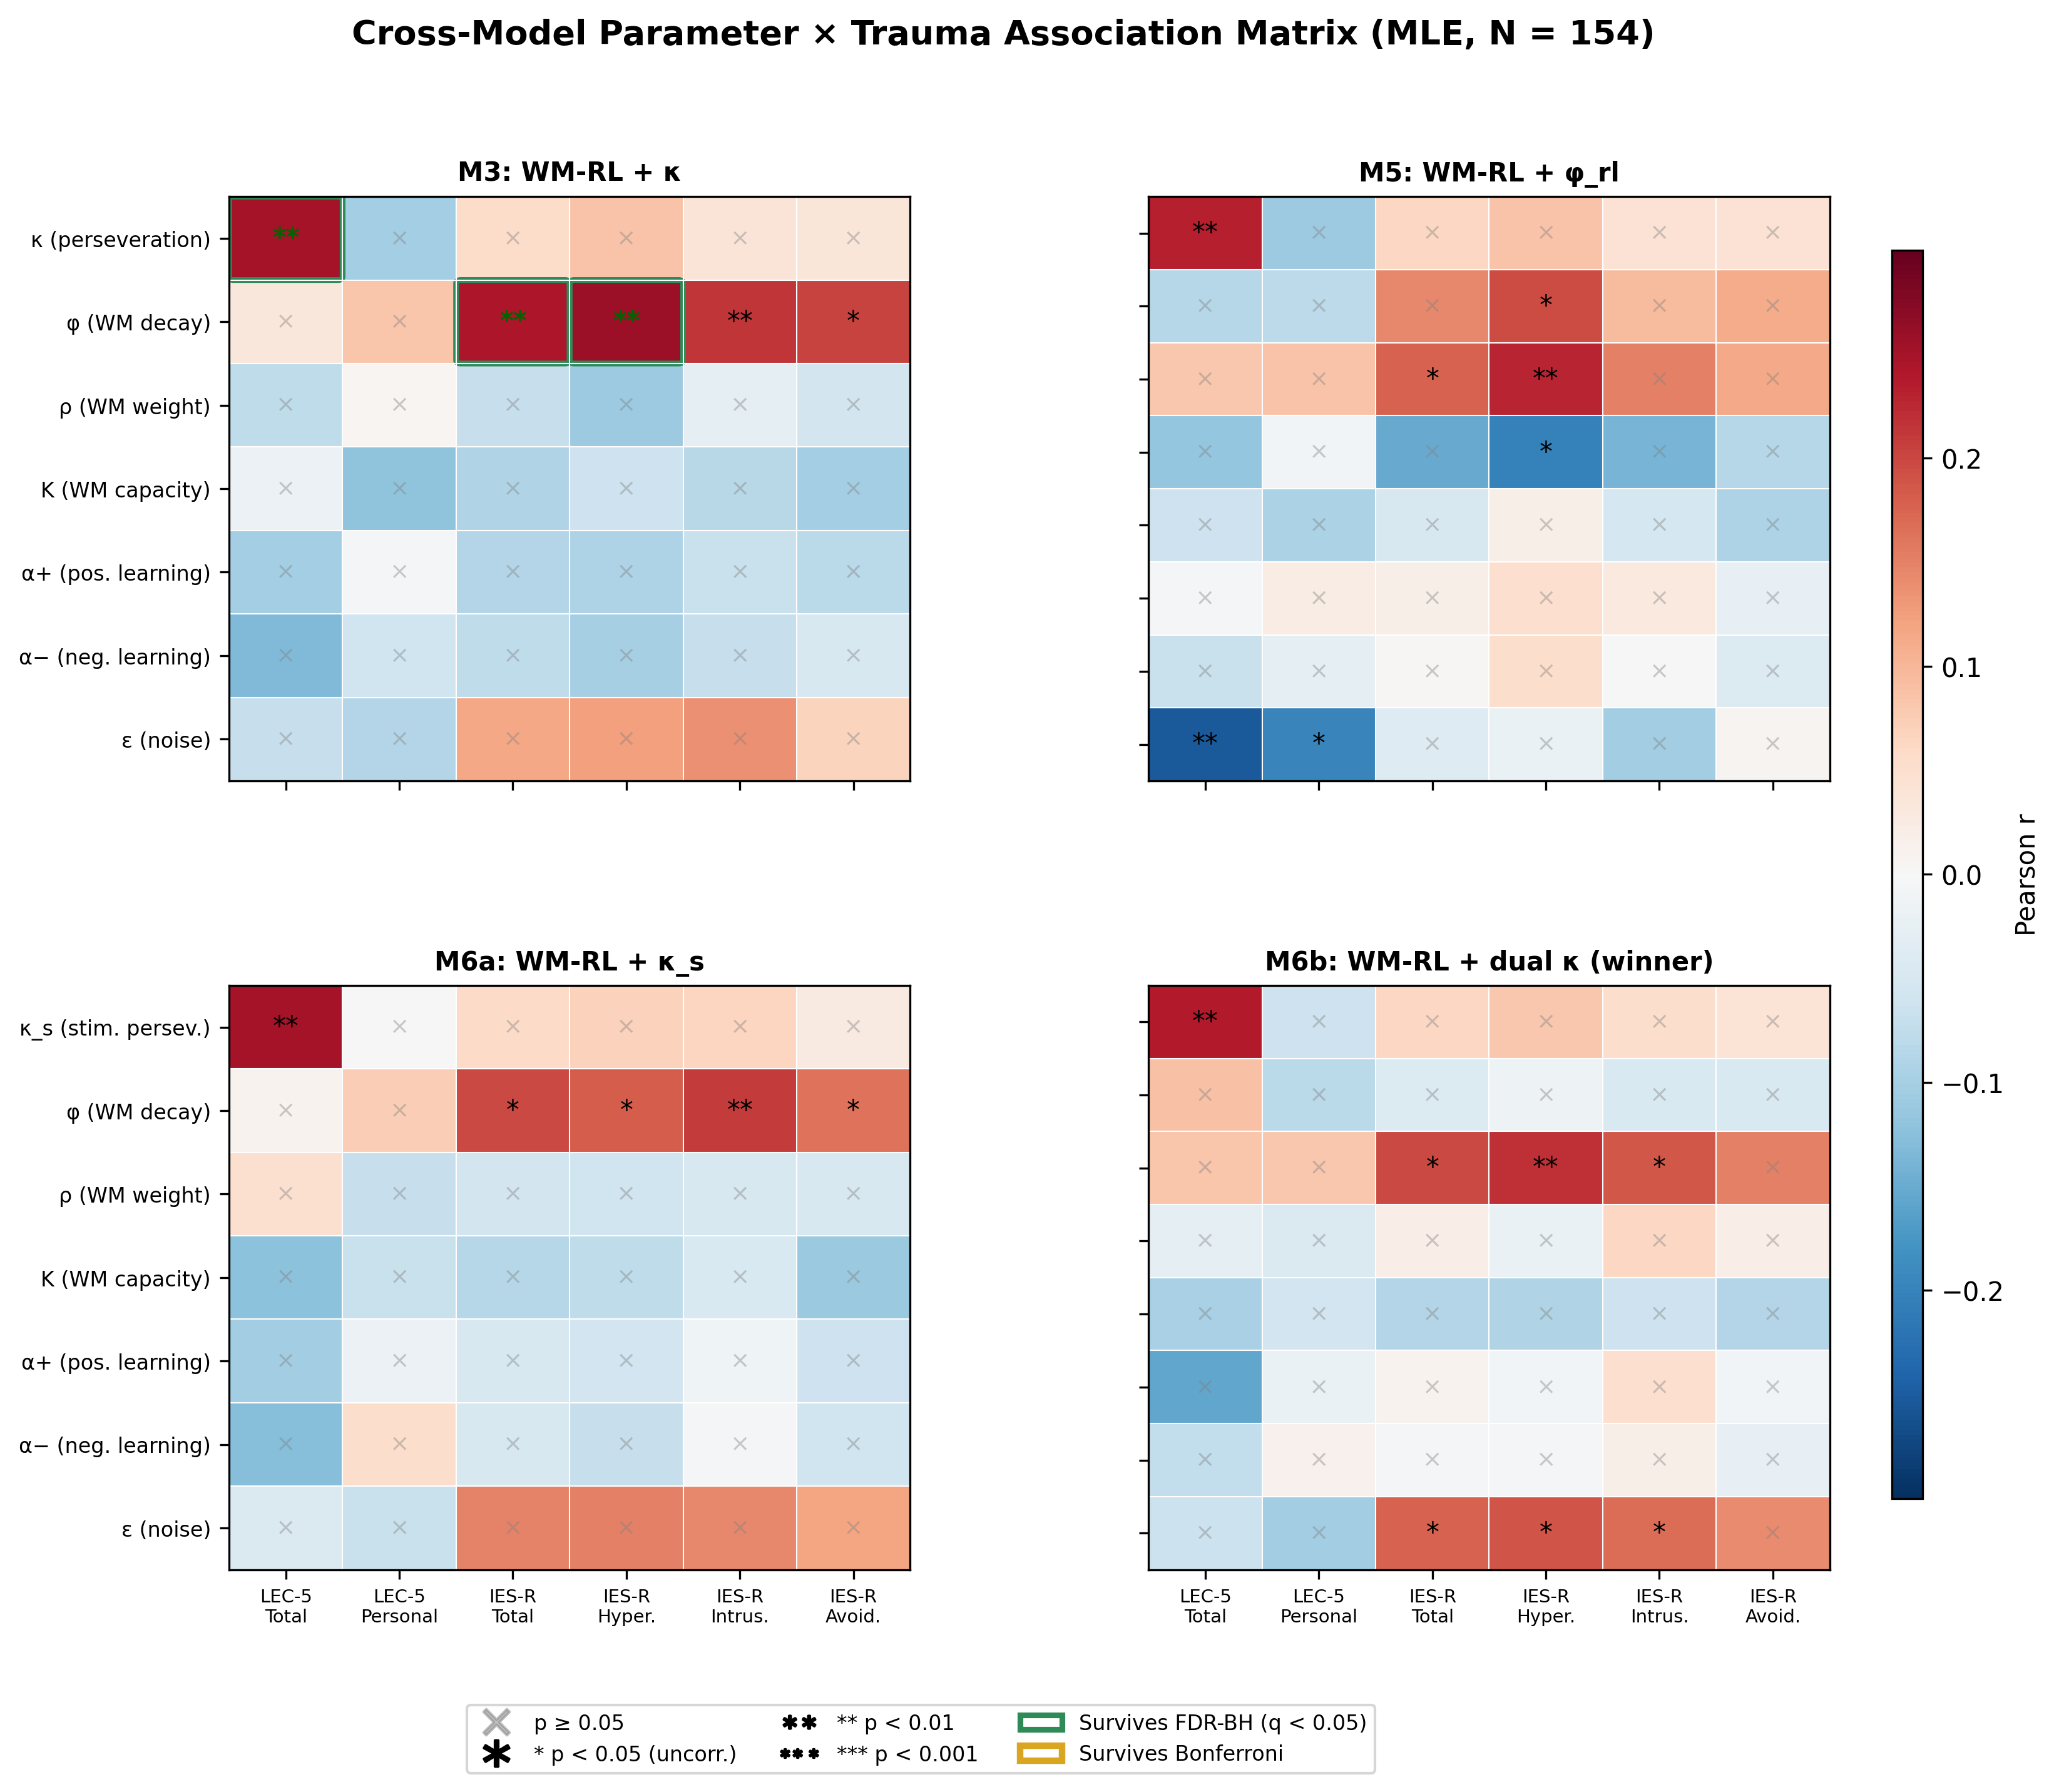
\includegraphics[width=1\linewidth,height=\textheight,keepaspectratio]{../reports/figures/model_comparison/cross_model_significance_heatmap.png}

}

\caption{\label{fig-cross-model-heatmap}Cross-model parameter \(\times\)
trauma association matrix. Each panel shows one WM-RL model variant (M3,
M5, M6a, M6b). See text for legend details.}

\end{figure}%

\subsection{Appendix J: Model Parameters}\label{sec-model-table}

\begin{longtable}[]{@{}llll@{}}

\caption{\label{tbl-model-params}Free parameters for all seven
computational models. M4 is the only joint choice+RT model; its AIC is
not comparable to choice-only models M1--M6b.}

\tabularnewline

\caption{}\label{T_20fea}\tabularnewline
\toprule\noalign{}
Model & Free Parameters & k & Type \\
\midrule\noalign{}
\endfirsthead
\toprule\noalign{}
Model & Free Parameters & k & Type \\
\midrule\noalign{}
\endhead
\bottomrule\noalign{}
\endlastfoot
M1: Q-Learning & alpha, epsilon & 2 & Choice only \\
M2: WM-RL & alpha, phi, rho, K, epsilon & 5 & Choice only \\
M3: WM-RL+kappa & alpha, phi, rho, K, kappa, epsilon & 6 & Choice
only \\
M5: WM-RL+phi\_rl & alpha, phi, rho, K, kappa, phi\_RL, epsilon & 7 &
Choice only \\
M6a: WM-RL+kappa\_s & alpha, phi, rho, K, kappa\_s, epsilon & 6 & Choice
only \\
M6b: WM-RL+dual & alpha, phi, rho, K, kappa\_total, kappa\_share,
epsilon & 7 & Choice only \\
M4: RLWM-LBA & alpha, phi, rho, K, kappa, v\_scale, A, delta, t0 & 9 &
Choice+RT \\

\end{longtable}

\subsection{Appendix K: Exclusion Criteria}\label{sec-exclusions}

All v4.0 analyses used a canonical cohort implemented as
\texttt{config.get\_analysis\_cohort()}. A participant was included if
\textbf{all three} of the following gates were satisfied:

\begin{enumerate}
\def\labelenumi{\arabic{enumi}.}
\tightlist
\item
  \textbf{Task completeness}. The participant contributed at least 400
  trials to the main task (blocks 3--23) and participated in at least 8
  main-task blocks. The trial-count threshold
  (\texttt{MIN\_TRIALS\_THRESHOLD\ =\ 400} in \texttt{config.py})
  corresponds to approximately 50\% of the expected 807--1077 trials
  across 21 blocks and ensures sufficient data for reliable parameter
  estimation.
\item
  \textbf{Performance check}. Overall accuracy \(\geq\) 0.40 AND mean
  accuracy across the last 5 main-task blocks \(\geq\) 0.50. With three
  response options, chance is \(1/3 \approx 0.333\). The
  overall-accuracy gate rules out participants at or below chance; the
  late-block gate additionally confirms that the participant
  \emph{learned} rather than performing at chance throughout the
  session. A participant who selected the correct response
  deterministically in a small minority of blocks but was otherwise
  random would satisfy the overall gate but fail the late-block gate.
\item
  \textbf{Scale completeness}. Non-missing values on every required
  survey column: LEC-5 total events, IES-R total, IES-R intrusion, IES-R
  avoidance, IES-R hyperarousal. Participants with any missing survey
  data were excluded from Level-2 regression analyses; this was also
  applied upstream to the MCMC fit for the hierarchical Bayesian
  pipeline so that individual-level posteriors and group-level
  regressions are estimated on an identical sample.
\end{enumerate}

Participants with known duplicate or corrupted data
(\texttt{MANUAL\_EXCLUSIONS} in \texttt{config.py}) were always excluded
regardless of gates 1--3.



\end{document}
